\documentclass[10pt,a4paper]{article}
\usepackage[margin=18mm]{geometry}
\usepackage[T1]{fontenc}
\usepackage{lmodern,graphicx,booktabs,array,amsmath,amssymb,float,caption,subcaption,multirow}
\usepackage[table]{xcolor}
\usepackage{tikz}
\usepackage[americanvoltages,siunitx]{circuitikz}
\usepackage{hyperref}
\usetikzlibrary{arrows.meta,positioning,fit,backgrounds,shapes.geometric,calc}
\hypersetup{colorlinks=true,urlcolor=blue,linkcolor=blue,citecolor=teal}
\setlength{\parindent}{0pt}\setlength{\parskip}{4.5pt}
\captionsetup{font=small,labelfont=bf}
\graphicspath{{figures/}{../design-report/figures/}{../building-block/figures/}{../dc-link/figures/}{../../simulation/sharing/}}
\newcommand{\uF}{\ensuremath{\mu}F}
\newcolumntype{L}[1]{>{\raggedright\arraybackslash}p{#1}}
\newcolumntype{C}[1]{>{\centering\arraybackslash}p{#1}}
\definecolor{pos}{RGB}{200,235,200}\definecolor{neg}{RGB}{245,200,200}\definecolor{mid}{RGB}{255,240,190}
%% generated by scripts/bb_losses.py
\newcommand{\Prated}{2.65}
\newcommand{\Pbudget}{13.3}
\newcommand{\Ipk}{141}
\newcommand{\CreqBlock}{78}
\newcommand{\CreqTotal}{233}
\newcommand{\CreqAlone}{236}
\newcommand{\CeffBlock}{77}
\newcommand{\dVshared}{3.0}
\newcommand{\dValone}{9.1}
\newcommand{\IlegHFworst}{50}
\newcommand{\IlegHFrated}{29}
\newcommand{\IthreeHF}{65}
\newcommand{\PcondTyp}{5.55}
\newcommand{\PcondMax}{7.40}
\newcommand{\PcondCold}{3.75}
\newcommand{\Pdead}{0.20}
\newcommand{\Pgate}{0.078}
\newcommand{\Pcap}{0.39}
\newcommand{\PcuHf}{1.07}
\newcommand{\PcuTot}{4.37}
\newcommand{\PcuHfLowM}{2.5}
\newcommand{\PcapOld}{0.08}
\newcommand{\Pcu}{3.30}
\newcommand{\Psw}{1.91}
\newcommand{\Ptot}{12.49}
\newcommand{\PcuOneOz}{4.67}
\newcommand{\PcuAC}{1.46}
\newcommand{\PcuDCP}{0.90}
\newcommand{\PcuDCN}{0.94}
\newcommand{\RacPath}{0.146}
\newcommand{\RdcpPath}{0.216}
\newcommand{\RdcnPath}{0.226}
\newcommand{\RdcpPathOneOz}{0.353}
\newcommand{\RdcnPathOneOz}{0.420}
\newcommand{\IdcpRms}{65}
\newcommand{\LloopTwoOz}{0.376}
\newcommand{\Eta}{99.53}
\newcommand{\EtaWorst}{99.46}
\newcommand{\PtotWorst}{14.34}
\newcommand{\Eavg}{38.1}
\newcommand{\Fmax}{60}
\newcommand{\Pdev}{1.91}
\newcommand{\Tj}{64}
\newcommand{\Idev}{35.4}
\newcommand{\LloopCu}{0.312}
\newcommand{\LloopEsl}{0.374}
\newcommand{\LloopLocalEsl}{0.399}
\newcommand{\LgateOne}{1.70}
\newcommand{\LgateBoth}{2.21}
\newcommand{\RhiPath}{0.369}
\newcommand{\RloPath}{0.413}
\newcommand{\CbootSel}{1}
\newcommand{\CbootMin}{680}
\newcommand{\BootDroop}{68}
\newcommand{\RgOn}{2}
\newcommand{\RgOff}{0}
\newcommand{\VdsH}{83.1}
\newcommand{\VdsL}{85.1}
\newcommand{\VgsBump}{0.98}
\newcommand{\VgsMin}{-1.29}
\newcommand{\EonPk}{47.4}
\newcommand{\EoffPk}{8.4}
\newcommand{\DvdtOn}{12}
\newcommand{\DvdtOff}{32}

% generated by scripts/design_report.py
\newcommand{\TotNone}{16.2}
\newcommand{\EtaNone}{99.39}
\newcommand{\PdevNone}{6.4}
\newcommand{\CondNone}{11.1}
\newcommand{\SwNone}{1.4}
\newcommand{\TotNtwo}{11.1}
\newcommand{\EtaNtwo}{99.58}
\newcommand{\PdevNtwo}{1.9}
\newcommand{\CondNtwo}{5.5}
\newcommand{\SwNtwo}{1.9}
\newcommand{\TotNthree}{9.8}
\newcommand{\EtaNthree}{99.63}
\newcommand{\PdevNthree}{1.0}
\newcommand{\CondNthree}{3.7}
\newcommand{\SwNthree}{2.4}
\newcommand{\TotNfour}{9.4}
\newcommand{\EtaNfour}{99.65}
\newcommand{\PdevNfour}{0.7}
\newcommand{\CondNfour}{2.8}
\newcommand{\SwNfour}{2.9}
\newcommand{\FoptSingle}{39}
\newcommand{\FoptInter}{26}
\newcommand{\LossOptSingle}{11.7}
\newcommand{\RipRmsFifty}{4.4}
\newcommand{\RipRmsTwenty}{11.1}
\newcommand{\Lph}{15}
\newcommand{\Rac}{15}
\newcommand{\Kfe}{0.6}
\newcommand{\Area}{8.5}
\newcommand{\PdArea}{0.31}
\newcommand{\PdVol}{764}
\newcommand{\Pmax}{3.05}
\newcommand{\PdAreaMax}{0.36}

% generated by scripts/design_report_v2.py
\newcommand{\DpuMax}{3.75}
\newcommand{\DpuTyp}{2.81}
\newcommand{\KanNHmm}{1.40}
\newcommand{\KqNHmm}{1.60}
\newcommand{\LfixNH}{0.18}
\newcommand{\LanCell}{0.14}
\newcommand{\DidtCell}{27}
\newcommand{\LloopMaxNine}{0.56}
\newcommand{\RoffMaxMin}{1.9}
\newcommand{\RoffMaxTyp}{2.7}
\newcommand{\RonTot}{3.0}
\newcommand{\RoffTot}{0.8}
\newcommand{\RdampMin}{0.97}
\newcommand{\ZetaOn}{2.2}
\newcommand{\ZetaOff}{0.58}
\newcommand{\VbumpMiller}{0.33}
\newcommand{\Fcross}{98}
\newcommand{\Icap}{2.5}
\newcommand{\NcapHundred}{12}
\newcommand{\AreaHundred}{6.2}
\newcommand{\Afixed}{4.2}
\newcommand{\RhoFifty}{0.31}
\newcommand{\RhoHundred}{0.42}
\newcommand{\EtaHundred}{99.45}
\newcommand{\RhoMaxCi}{0.42}
\newcommand{\RthHsFifty}{7.3}
\newcommand{\RthHsFiftyCool}{9.9}
\newcommand{\Rtim}{1.9}
\newcommand{\UtilBump}{89}
\newcommand{\UtilRipple}{100}
\newcommand{\UtilVds}{67}
\newcommand{\UtilWorst}{108}
\newcommand{\Tone}{10.7}
\newcommand{\CdptTwo}{575}
\newcommand{\CdptFive}{233}
\newcommand{\Fring}{258}
\newcommand{\Trise}{2.4}
\newcommand{\LreqTwentyFive}{53}
\newcommand{\LreqFifty}{27}
\newcommand{\LreqHundred}{13}

% generated by scripts/loss_characterization.py
\newcommand{\LcEonPk}{43}
\newcommand{\LcEoffPk}{8.1}
\newcommand{\LcEonZero}{12}
\newcommand{\LcPon}{1.53}
\newcommand{\LcPoff}{0.38}
\newcommand{\LcTotSeventyFive}{11.9}
\newcommand{\LcEtaSeventyFive}{99.55}
\newcommand{\LcEtaMaxSeventyFive}{99.49}
\newcommand{\LcCondSeventyFive}{4.97}
\newcommand{\LcTotHundred}{12.5}
\newcommand{\LcEtaHundred}{99.53}
\newcommand{\LcEtaMaxHundred}{99.46}
\newcommand{\LcCondHundred}{5.58}
\newcommand{\LcTotOneTwentyFive}{13.1}
\newcommand{\LcEtaOneTwentyFive}{99.51}
\newcommand{\LcEtaMaxOneTwentyFive}{99.43}
\newcommand{\LcCondOneTwentyFive}{6.18}
\newcommand{\LcTotOneFifty}{13.7}
\newcommand{\LcEtaOneFifty}{99.48}
\newcommand{\LcEtaMaxOneFifty}{99.40}
\newcommand{\LcCondOneFifty}{6.79}
\newcommand{\LcEonZeroFit}{12}
\newcommand{\LcQossV}{17}
\newcommand{\LcOvOnPk}{37}
\newcommand{\LcEonMinusZeroPk}{35}
\newcommand{\LcOvOffPk}{14}
\newcommand{\LcEoffMeasPk}{8.4}
\newcommand{\LcIpkMeas}{157}
\newcommand{\LcDvOnPk}{12}
\newcommand{\LcDvOffPk}{32}

% generated by scripts/slow_switching.py
\newcommand{\SlowCoss}{5.3}
\newcommand{\SlEonBase}{40.9}
\newcommand{\SlEoffBase}{8.0}
\newcommand{\SlFoffBase}{41.2}
\newcommand{\SlDvOffBase}{27}
\newcommand{\SlDvOnBase}{13}
\newcommand{\SlVdsBase}{86.5}
\newcommand{\SlBumpBase}{0.99}
\newcommand{\SlIdpkBase}{254}
\newcommand{\SlPswBase}{1.87}
\newcommand{\SlEtaBase}{99.53}
\newcommand{\SlTotBase}{12.5}
\newcommand{\SlEonOffTwo}{40.9}
\newcommand{\SlEoffOffTwo}{18.5}
\newcommand{\SlFoffOffTwo}{53.0}
\newcommand{\SlDvOffOffTwo}{15}
\newcommand{\SlDvOnOffTwo}{13}
\newcommand{\SlVdsOffTwo}{85.4}
\newcommand{\SlBumpOffTwo}{1.10}
\newcommand{\SlIdpkOffTwo}{254}
\newcommand{\SlPswOffTwo}{2.16}
\newcommand{\SlEtaOffTwo}{99.52}
\newcommand{\SlTotOffTwo}{12.7}
\newcommand{\SlEonOffFive}{40.9}
\newcommand{\SlEoffOffFive}{39.6}
\newcommand{\SlFoffOffFive}{82.1}
\newcommand{\SlDvOffOffFive}{9}
\newcommand{\SlDvOnOffFive}{13}
\newcommand{\SlVdsOffFive}{86.6}
\newcommand{\SlBumpOffFive}{1.21}
\newcommand{\SlIdpkOffFive}{254}
\newcommand{\SlPswOffFive}{2.76}
\newcommand{\SlEtaOffFive}{99.50}
\newcommand{\SlTotOffFive}{13.3}
\newcommand{\SlEonOffTen}{41.0}
\newcommand{\SlEoffOffTen}{78.7}
\newcommand{\SlFoffOffTen}{138.5}
\newcommand{\SlDvOffOffTen}{5}
\newcommand{\SlDvOnOffTen}{13}
\newcommand{\SlVdsOffTen}{85.2}
\newcommand{\SlBumpOffTen}{1.29}
\newcommand{\SlIdpkOffTen}{254}
\newcommand{\SlPswOffTen}{3.92}
\newcommand{\SlEtaOffTen}{99.46}
\newcommand{\SlTotOffTen}{14.5}
\newcommand{\SlEonOnTen}{102.4}
\newcommand{\SlEoffOnTen}{18.5}
\newcommand{\SlFoffOnTen}{53.0}
\newcommand{\SlDvOffOnTen}{15}
\newcommand{\SlDvOnOnTen}{11}
\newcommand{\SlVdsOnTen}{85.4}
\newcommand{\SlBumpOnTen}{0.94}
\newcommand{\SlIdpkOnTen}{195}
\newcommand{\SlPswOnTen}{4.08}
\newcommand{\SlEtaOnTen}{99.45}
\newcommand{\SlTotOnTen}{14.7}
\newcommand{\SlEonBoth}{102.8}
\newcommand{\SlEoffBoth}{78.6}
\newcommand{\SlFoffBoth}{138.4}
\newcommand{\SlDvOffBoth}{5}
\newcommand{\SlDvOnBoth}{11}
\newcommand{\SlVdsBoth}{85.3}
\newcommand{\SlBumpBoth}{1.20}
\newcommand{\SlIdpkBoth}{195}
\newcommand{\SlPswBoth}{5.86}
\newcommand{\SlEtaBoth}{99.38}
\newcommand{\SlTotBoth}{16.4}


\tikzset{
  blk/.style={draw,rounded corners=2pt,fill=blue!6,align=center,minimum height=0.9cm,font=\small},
  tool/.style={draw,rounded corners=2pt,fill=orange!12,align=center,minimum height=0.9cm,font=\small},
  dec/.style={draw,diamond,aspect=2.2,fill=green!10,align=center,font=\small,inner sep=1pt},
  hw/.style={draw,rounded corners=2pt,fill=gray!12,align=center,minimum height=0.9cm,font=\small},
  arr/.style={-{Latex[length=2mm]},thick},
}

\title{\textbf{Design Report}\\[4pt]\large Methodology and Design of a Paralleled-GaN Phase-Leg Building Block\\for Stacked Polyphase Bridge Traction Drives\\[3pt]\normalsize 75\,V DC link $\cdot$ 100\,A$_\mathrm{rms}$ $\cdot$ 2\,$\times$\,EPC2361 per switch $\cdot$ symmetric centre-driver layout}
\author{PCB-Design project, KTH}
\date{7 October 2026 --- design phase (analysis, Ansys Q3D and LTspice; hardware pending)}

\begin{document}
\maketitle

\begin{abstract}
\noindent This report presents the design of a GaN phase-leg building block for stacked polyphase bridge (SPB) traction drives, structured after the design methodologies of recent paralleled-GaN inverter and power-module publications~\cite{tran2025,zou2025,cooke2026,wattenberg2023,lu2017,brothers2019}.
The design is formulated as a multi-objective problem (efficiency, power density, switching frequency, voltage stress, current sharing, gate robustness) and solved in a model-based framework: analytical sizing, a parametric layout that drives Ansys Q3D extraction, LTspice switching simulation with the extracted $RLK$ matrix, and loss, thermal and DC-link models that close the loop to the switching-frequency choice.
The result is a 30\,$\times$\,28\,mm four-layer block with two mirrored commutation cells and a centre gate driver: 0.37\,nH commutation loop per cell (Q3D, copper + MLCC ESL; package inductance not included), \LgateOne\,nH matched gate loops, $<$\,0.1\,\% predicted current imbalance, peak $V_\mathrm{DS}$ of \VdsL\,V at 160\,A with R$_\mathrm{g,on}$/R$_\mathrm{g,off}$\,=\,\RgOn/\RgOff\,$\Omega$, and \Eta\,\% efficiency at 50\,kHz (\EtaHundred\,\% at 100\,kHz) for \Prated\,kW per leg.
The report also identifies where the design is close to its limits: the DC-link ripple, the high-side gate bump, and the loss. A Q3D frequency sweep shows \PcuHf\,W of copper loss at the switching harmonics, which leaves little margin at 50\,kHz and puts the worst-case on-resistance case and 100\,kHz above the budget.
\end{abstract}

\vspace{-2mm}
\begin{table}[H]\centering\small
\caption{Design specification and key results.}
\begin{tabular}{@{}L{6.6cm}L{3.9cm}L{6.0cm}@{}}\toprule
Quantity & Value & Basis \\\midrule
DC link / phase current / rated power per leg & 75\,V / 100\,A$_\mathrm{rms}$ (\Ipk\,A$_\mathrm{pk}$) / \Prated\,kW & specification; $M=1$, $\cos\varphi=1$ \\
Switching frequency & 50\,kHz nominal (target met up to \Fmax\,kHz) & Sections~\ref{sec:loss}, \ref{sec:coopt} \\
Devices & 2\,$\times$\,EPC2361 (100\,V, 0.75/1.0\,m$\Omega$) per switch & Section~\ref{sec:device} \\
Commutation loop per cell & \LloopEsl\,nH (incl.\ MLCC ESL, excl.\ package) & Q3D, Section~\ref{sec:loop} \\
Gate loop per FET & \LgateOne\,nH, symmetric & Q3D, Section~\ref{sec:gate} \\
Gate resistors on / off & \RgOn\,/\,\RgOff\,$\Omega$ ($\zeta_\mathrm{on}$ = \ZetaOn) & LTspice sweep + design window \\
Peak $V_\mathrm{DS}$ at 160\,A; dv/dt on/off & \VdsH\,/\,\VdsL\,V; \DvdtOn\,/\,\DvdtOff\,V/ns & LTspice with Q3D parasitics \\
Loss / efficiency at 50\,kHz & \Ptot\,W / \Eta\,\% (\EtaWorst\,\% max $R_\mathrm{DS(on)}$) & Section~\ref{sec:loss} \\
DC link per leg & 24\,$\times$\,10\,\uF{} 1210 + 12\,$\times$\,1\,\uF{} 0805 (\CeffBlock\,\uF{} eff.) & Section~\ref{sec:dclink} \\
Board area, power density (board level) & \Area\,cm$^2$, \PdArea\,kW/cm$^2$ & Section~\ref{sec:coopt} \\
\bottomrule\end{tabular}\end{table}

\tableofcontents
\newpage

%=====================================================================
\section{Introduction}
%=====================================================================
\subsection{Motivation: why a low-voltage GaN building block for high-voltage traction}
In a stacked polyphase bridge (SPB) the DC bus is divided into $N$ series-connected modules, each supplying its own group of phases of a multiphase machine and seeing only $V_\mathrm{dc}/N$.
For an 800\,V bus and 75\,V modules ($N\approx11$), 100\,V GaN HEMTs can be used: they have the lowest $R_\mathrm{DS(on)}\cdot Q_\mathrm{G}$ figure of merit, no reverse recovery, and chip-scale packages with sub-nH package inductance.
The low voltage step per module also reduces the winding insulation stress compared with a full-bus SiC inverter.
Three-level GaN inverters~\cite{satpathy2022} pursue a similar goal with 650\,V devices.
Because one building block is repeated $N$ times, its efficiency, density and robustness multiply at system level.

\subsection{Design challenges identified in the literature}
\begin{itemize}\itemsep1pt
\item \textbf{Current capability} of a single GaN die is limited, so devices must be paralleled~\cite{zou2025,cooke2026,wattenberg2023,tran2025}.
\item \textbf{Voltage overshoot} is the primary failure mechanism of low-voltage GaN modules. A commercial 100\,V, 270\,A-per-phase module failed at 292\,A, 36\,\% of its die rating, because of its package inductance~\cite{brothers2019}.
\item \textbf{Asymmetric loops} give unequal dynamic current sharing. Lateral loops and cascaded phases give 11--28\,nH unequal loops~\cite{brothers2019}. Mismatched quasi-common-source inductance and power-to-gate coupling are the most critical factors~\cite{tran2025,lu2017}.
\item \textbf{Fragile gates}: $V_\mathrm{GS,max}$ is +6\,V and $V_\mathrm{th}$ is about 1\,V, so gate ringing and Miller bumps must be controlled~\cite{tran2025,lu2017,musumeci2022}.
\item \textbf{Efficiency and density} trade off through the switching frequency, the DC link and the heat sink, so they must be co-optimised rather than optimised separately~\cite{zou2025}.
\end{itemize}

\subsection{Approach and contributions of this design}
\begin{enumerate}\itemsep1pt
\item A model-based design framework (Fig.~\ref{fig:framework}) in which a single parametric geometry drives the layout drawings, the Q3D extraction and the SPICE netlist. Every number in this report can be regenerated.
\item A symmetric ``butterfly'' building block in the spirit of~\cite{wattenberg2023}: two mirrored vertical commutation cells, a centre gate driver with equal gate stars and Kelvin returns, and a distributed MLCC bank.
\item Quantified design rules: a gate-resistor design window, an overshoot design space, a current-sharing sensitivity ranking, and DC-link and thermal bounds versus $f_\mathrm{sw}$.
\item A board-level efficiency--density--$f_\mathrm{sw}$ analysis following~\cite{zou2025}, and a winding-ripple requirement that can be handed to the machine design.
\end{enumerate}

%=====================================================================
\section{State of the art}\label{sec:sota}
%=====================================================================
Table~\ref{tab:sota} and Fig.~\ref{fig:benchmark} summarise the reviewed paralleled-GaN half bridges.
Two layout families stand out.
PCB-based vertical (flux-cancelling) loops reach sub-nH inductance~\cite{lu2017,cooke2026}.
DBC, IMS and module solutions trade inductance for thermal performance: 1.1--6.4\,nH~\cite{tran2025,zou2025,rahman2025,novo2024}.
The device power utilisation (DPU) of~\cite{cooke2026},
\begin{equation}
\mathrm{DPU}=\frac{V_\mathrm{dc}\,I_\mathrm{ph}}{n\,V_\mathrm{DS}^2/R_\mathrm{DS(on)}}\cdot10^4,
\end{equation}
is \DpuMax{} for this design ($R_\mathrm{DS(on),max}$; \DpuTyp{} with the typical value).
This is comparable to the continuously operated inverters in~\cite{cooke2026} (2.3--9.5).
Note that our value is a design point, not a test result.

\begin{table}[H]\centering\footnotesize
\caption{Reviewed paralleled-GaN half-bridge designs (values as reported; loop definitions differ between papers).}\label{tab:sota}
\setlength{\tabcolsep}{3pt}\begin{tabular}{@{}L{3.0cm}L{2.5cm}L{2.2cm}L{1.4cm}L{2.2cm}L{5.0cm}@{}}\toprule
Work & Devices per switch & Test & $L_\mathrm{loop}$ & Gate drive & Key design features \\\midrule
Lu \& Chen 2017~\cite{lu2017} & 4\,$\times$\,GS66516T (650\,V) & DPT 400\,V/240\,A & 0.7\,nH & one driver, symmetric & 6-layer PCB, quasi-CSI $<$0.2\,nH, analytic switching model \\
Brothers 2019~\cite{brothers2019} & 4\,$\times$\,GS61008 (100\,V) & DPT 48\,V/367\,A & -- & 10/4\,$\Omega$ per die & flux-cancelling PCB; commercial module failed at 292\,A \\
Wattenberg 2023~\cite{wattenberg2023} & 8\,$\times$\,100\,V 3\,m$\Omega$ & 3-ph 48\,V, 125\,A$_\mathrm{rms}$ & -- & centre driver, $R_G$ 1\,$\Omega$ & ``butterfly'' layout, gate loops $\approx$1\,nH within 17\,\%, MLCC DC link \\
Musumeci 2022~\cite{musumeci2022} & 2\,$\times$\,EPC2065 (80\,V) & motor 48\,V/35\,A & -- & 10\,$\Omega$ & $V_\mathrm{th}$ spread identified as the most critical parameter \\
Palma 2024~\cite{palma2024} & 4\,$\times$\,EPC2302 (100\,V) & motor 60\,V/150\,A$_\mathrm{rms}$ & -- & one driver/leg & 12-device characterisation board, peak-current prediction \\
Satpathy 2022~\cite{satpathy2022} & 2\,$\times$\,GS66516B (650\,V) & 3L-ANPC 550\,V, 70\,kHz & 6.3\,nH & split $R_\mathrm{on}/R_\mathrm{off}$ & IMS + capacitor PCB, PLECS thermal \\
Novo 2024~\cite{novo2024} & 4\,$\times$\,D3GaN (650\,V) & WLTP 350\,A$_\mathrm{rms}$ & 3.9\,nH & drivers above devices & turn-on skew 2.8\,ns, 99.3\,\% \\
Tran 2025~\cite{tran2025} & 4\,$\times$\,GS61008P (100\,V) & DPT 48\,V/328\,A, 5\,kW & 1.14\,nH & Si8271, 4.7/4\,$\Omega$ & IMS hybrid, Q3D$\to$LTspice$\to$Icepak framework \\
Zou 2025~\cite{zou2025} & 3\,$\times$\,V08TC65 (650\,V) & 100\,kW inverter & 6.4\,nH & integrated, 1.4\,nH & $\eta$--$\rho$--$f_\mathrm{sw}$ Pareto co-optimisation \\
Rahman 2025~\cite{rahman2025} & 2\,$\times$\,GS-065-150 (650\,V) & DPT 350\,V & 5.52\,nH & co-packaged & multilayer substrate, 40\,\% lower $L$ \\
Cooke 2026~\cite{cooke2026} & 8\,$\times$\,EPC2304 (200\,V) & 120\,V/155\,A, 100\,kHz & 0.34\,nH (est.) & 15/2\,$\Omega$, $+5.3/-3$\,V & symmetric gate PCB, thermal-image sharing check \\
\rowcolor{red!6}\textbf{This design} & 2\,$\times$\,EPC2361 (100\,V) & design 75\,V/141\,A & 0.37\,nH/cell & LT8418 centre, 2/0\,$\Omega$ & mirrored cells, Q3D$\to$LTspice, $\eta$--$\rho$--$f_\mathrm{sw}$ incl.\ machine \\
\bottomrule\end{tabular}\end{table}

\begin{figure}[H]\centering
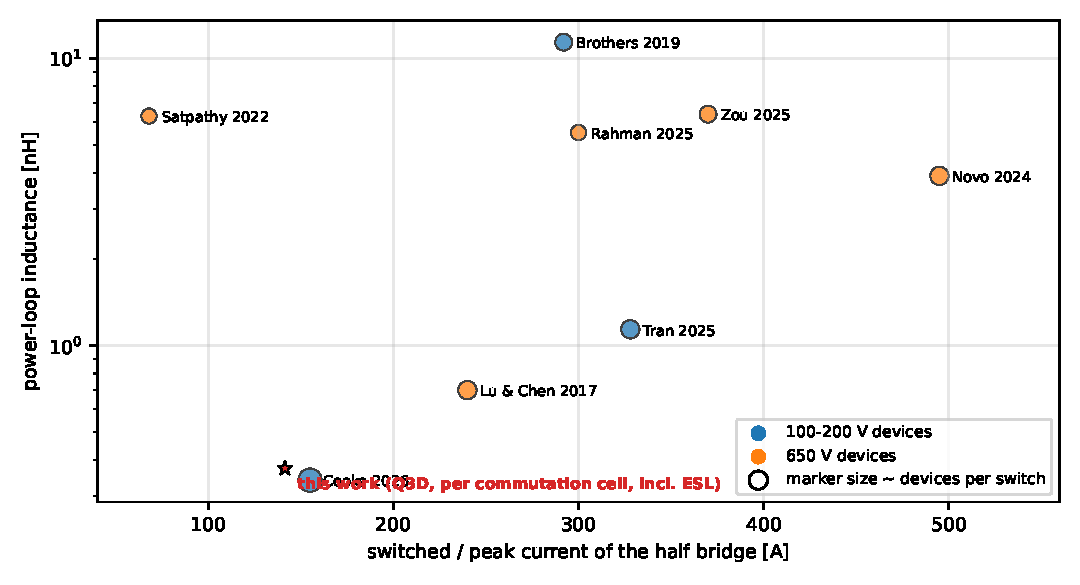
\includegraphics[width=0.78\textwidth]{benchmark.pdf}
\caption{Power-loop inductance versus switched current for the reviewed designs. Low-voltage, high-current designs must sit at the lower right because $\Delta V=L\,di/dt$ has to fit into a 10--25\,V margin.}\label{fig:benchmark}
\end{figure}

%=====================================================================
\section{Design objectives, constraints and methodology}\label{sec:method}
%=====================================================================
\subsection{Objectives and constraints}
\begin{table}[H]\centering\small
\caption{Objectives and hard constraints.}
\begin{tabular}{@{}L{3.7cm}L{6.4cm}L{6.4cm}@{}}\toprule
 & Metric & Target / limit \\\midrule
Efficiency & loss per leg at the rated point & $\leq$\,\Pbudget\,W ($\eta\geq99.5$\,\%) \\
Switching frequency & highest $f_\mathrm{sw}$ meeting the efficiency target & $\geq$\,50\,kHz; 100\,kHz desirable \\
Winding ripple & $\Delta i_\mathrm{pp}\approx V_\mathrm{dc}/(4Lf_\mathrm{sw})$ & requirement to the machine design (Section~\ref{sec:loss}) \\
Power density & board area per kW (board level) & maximise \\
Voltage stress & peak $V_\mathrm{DS}$ (rating 100\,V, 120\,V repetitive transient) & $\leq$\,90\,V at 160\,A (13\,\% overload) \\
Gate robustness & $V_\mathrm{GS}$ overshoot, Miller bump, negative excursion & $<$\,6\,V; bump $\leq$\,1\,V; $>$\,$-4$\,V \\
Current sharing & dynamic and static imbalance & as small as the layout allows \\
Measurability & DPT access to $V_\mathrm{DS}$, $V_\mathrm{GS}$ and device current & test points without adding loop inductance \\
\bottomrule\end{tabular}\end{table}

\subsection{Trade-off matrix}
Table~\ref{tab:tradeoff} shows how each design variable acts on the objectives. Green means favourable, red unfavourable, yellow weak or mixed.
It is the qualitative map that the following sections quantify.

\begin{table}[H]\centering\footnotesize
\caption{Effect of increasing each design variable on the objectives.}\label{tab:tradeoff}
\setlength{\tabcolsep}{3pt}
\begin{tabular}{@{}L{3.6cm}C{1.6cm}C{1.6cm}C{1.6cm}C{1.6cm}C{1.6cm}C{1.6cm}C{1.6cm}@{}}\toprule
Increase of \dots & Inverter loss & Winding ripple & Density & $V_\mathrm{DS}$ peak & Sharing risk & Gate bump & Cost \\\midrule
$f_\mathrm{sw}$ & \cellcolor{neg}$\uparrow$ & \cellcolor{pos}$\downarrow$ & \cellcolor{pos}$\uparrow$ (DC link) & \cellcolor{mid}-- & \cellcolor{mid}-- & \cellcolor{mid}-- & \cellcolor{mid}-- \\
devices in parallel $n$ & \cellcolor{pos}$\downarrow$ cond., \cellcolor{neg}$\uparrow$ $Q_\mathrm{oss}$ & \cellcolor{mid}-- & \cellcolor{neg}$\downarrow$ & \cellcolor{neg}$\uparrow$ (longer loop) & \cellcolor{neg}$\uparrow$ & \cellcolor{mid}-- & \cellcolor{neg}$\uparrow$ \\
L1--L2 dielectric $h$ & \cellcolor{mid}-- & \cellcolor{mid}-- & \cellcolor{mid}-- & \cellcolor{neg}$\uparrow$ & \cellcolor{mid}-- & \cellcolor{mid}-- & \cellcolor{pos}$\downarrow$ \\
$R_\mathrm{g,on}$ & \cellcolor{neg}$\uparrow E_\mathrm{on}$ & \cellcolor{mid}-- & \cellcolor{mid}-- & \cellcolor{pos}$\downarrow$ (HS) & \cellcolor{pos}$\downarrow$ & \cellcolor{pos}$\downarrow$ & \cellcolor{mid}-- \\
$R_\mathrm{g,off}$ & \cellcolor{mid}small & \cellcolor{mid}-- & \cellcolor{mid}-- & \cellcolor{mid}small & \cellcolor{mid}-- & \cellcolor{neg}$\uparrow$ & \cellcolor{mid}-- \\
copper weight (oz) & \cellcolor{pos}$\downarrow$ & \cellcolor{mid}-- & \cellcolor{mid}-- & \cellcolor{mid}slight $\uparrow$ & \cellcolor{mid}-- & \cellcolor{mid}-- & \cellcolor{neg}$\uparrow$ \\
DC-link capacitance & \cellcolor{mid}ESR $\downarrow$ & \cellcolor{mid}-- & \cellcolor{neg}$\downarrow$ & \cellcolor{pos}$\downarrow$ (ringing) & \cellcolor{mid}-- & \cellcolor{mid}-- & \cellcolor{neg}$\uparrow$ \\
gate-loop asymmetry & \cellcolor{neg}$\uparrow$ & \cellcolor{mid}-- & \cellcolor{mid}-- & \cellcolor{mid}-- & \cellcolor{neg}$\uparrow\uparrow$ & \cellcolor{neg}$\uparrow$ & \cellcolor{mid}-- \\
\bottomrule\end{tabular}\end{table}

\subsection{Model-based design framework}
Following the digital framework of~\cite{tran2025} and the co-optimisation flow of~\cite{zou2025}, the design is carried out in the loop shown in Fig.~\ref{fig:framework}.
Unlike a layout-first flow, the geometry is a parametric Python description (\texttt{bb\_geometry.py}). That one description generates the layout drawings, the Q3D model and therefore the SPICE parasitics, so a change of, for example, the dielectric thickness propagates to losses and overshoot without manual steps.

\begin{figure}[H]\centering
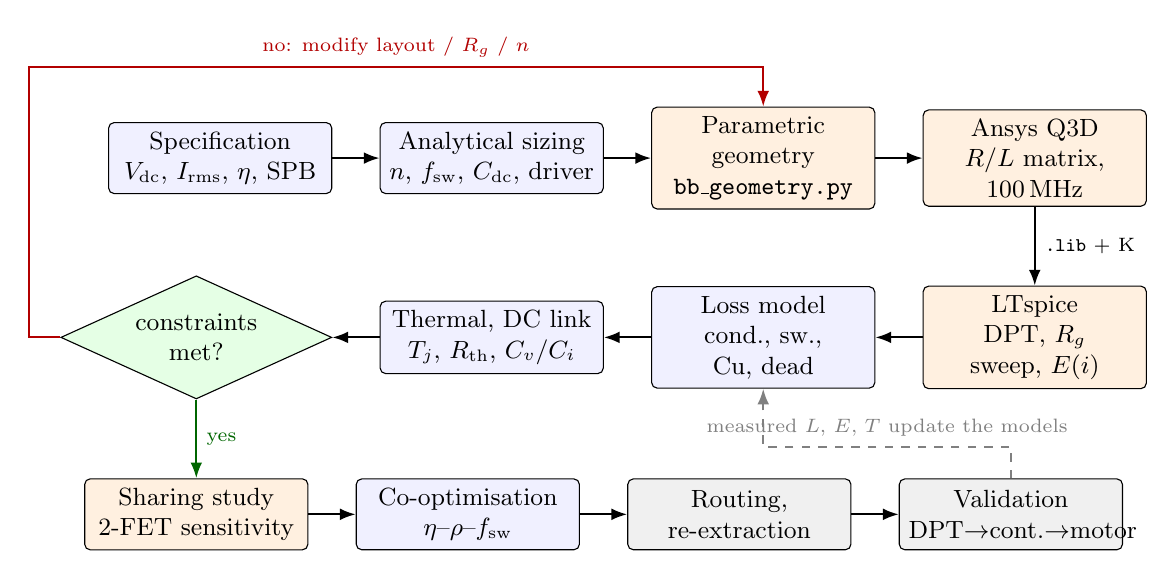
\begin{tikzpicture}[node distance=5mm and 6mm]
\node[blk,text width=2.6cm] (spec) {Specification\\$V_\mathrm{dc}$, $I_\mathrm{rms}$, $\eta$, SPB};
\node[blk,text width=2.6cm,right=of spec] (an) {Analytical sizing\\$n$, $f_\mathrm{sw}$, $C_\mathrm{dc}$, driver};
\node[tool,text width=2.6cm,right=of an] (geo) {Parametric geometry\\\texttt{bb\_geometry.py}};
\node[tool,text width=2.6cm,right=of geo] (q3d) {Ansys Q3D\\$R/L$ matrix, 100\,MHz};
\node[tool,text width=2.6cm,below=10mm of q3d] (sp) {LTspice\\DPT, $R_g$ sweep, $E(i)$};
\node[blk,text width=2.6cm,left=of sp] (loss) {Loss model\\cond., sw., Cu, dead};
\node[blk,text width=2.6cm,left=of loss] (th) {Thermal, DC link\\$T_j$, $R_\mathrm{th}$, $C_v/C_i$};
\node[dec,text width=1.9cm,left=of th] (ok) {constraints\\met?};
\node[tool,text width=2.6cm,below=10mm of ok] (sh) {Sharing study\\2-FET sensitivity};
\node[blk,text width=2.6cm,right=of sh] (co) {Co-optimisation\\$\eta$--$\rho$--$f_\mathrm{sw}$};
\node[hw,text width=2.6cm,right=of co] (pcb) {Routing,\\re-extraction};
\node[hw,text width=2.6cm,right=of pcb] (test) {Validation\\DPT$\to$cont.$\to$motor};
\draw[arr] (spec)--(an); \draw[arr] (an)--(geo); \draw[arr] (geo)--(q3d);
\draw[arr] (q3d)--node[right,font=\scriptsize]{\texttt{.lib} + K} (sp);
\draw[arr] (sp)--(loss); \draw[arr] (loss)--(th); \draw[arr] (th)--(ok);
\draw[arr,red!70!black] (ok.west) -- ++(-4mm,0) |- node[pos=0.75,above,font=\scriptsize]{no: modify layout / $R_g$ / $n$} ($(geo.north)+(0,5mm)$) -- (geo.north);
\draw[arr,green!40!black] (ok.south) -- node[right,font=\scriptsize]{yes} (sh.north);
\draw[arr] (sh)--(co); \draw[arr] (co)--(pcb); \draw[arr] (pcb)--(test);
\draw[arr,dashed,gray] (test.north) -- ++(0,4mm) -| node[pos=0.25,above,font=\scriptsize]{measured $L$, $E$, $T$ update the models} (loss.south);
\end{tikzpicture}
\caption{Design framework. Orange: field and circuit solvers; blue: analytical models; grey: hardware steps (pending).}\label{fig:framework}
\end{figure}

%=====================================================================
\section{System architecture}\label{sec:arch}
%=====================================================================
\begin{figure}[H]\centering
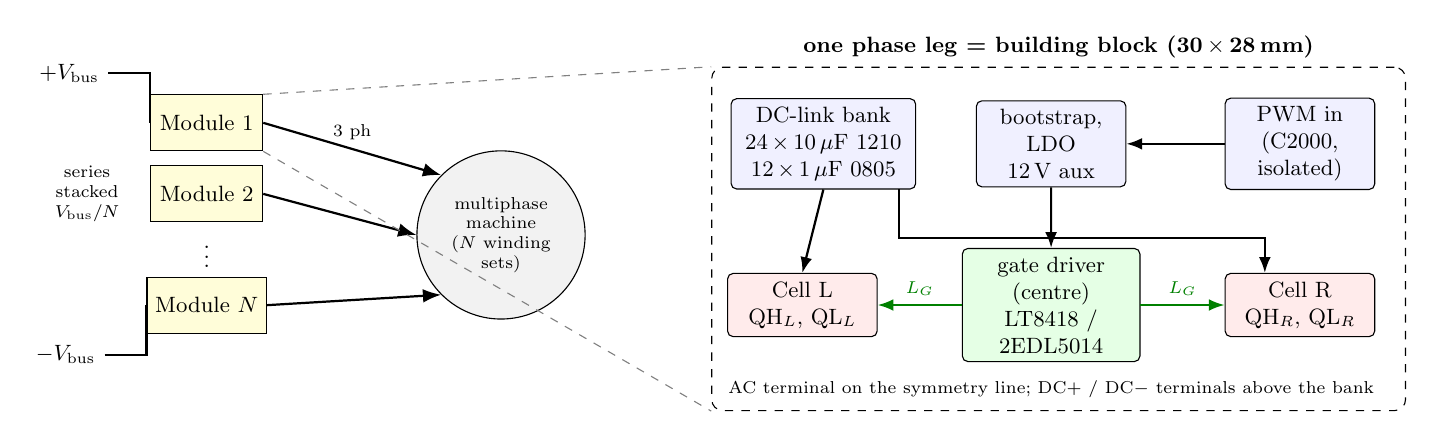
\begin{tikzpicture}[node distance=3mm and 4mm,font=\small,scale=0.89,transform shape]
% SPB stack
\node[draw,fill=yellow!15,minimum width=1.6cm,minimum height=0.8cm] (m1) at (0,0) {Module 1};
\node[draw,fill=yellow!15,minimum width=1.6cm,minimum height=0.8cm,below=2mm of m1] (m2) {Module 2};
\node[below=0mm of m2] (dots) {$\vdots$};
\node[draw,fill=yellow!15,minimum width=1.6cm,minimum height=0.8cm,below=0mm of dots] (mn) {Module $N$};
\draw[thick] ($(m1.north west)+(-0.6,0.3)$) node[left]{$+V_\mathrm{bus}$} -- ++(0.6,0) |- (m1.west);
\draw[thick] ($(mn.south west)+(-0.6,-0.3)$) node[left]{$-V_\mathrm{bus}$} -- ++(0.6,0) |- (mn.west);
\node[font=\scriptsize,align=center] at ($(m2.west)+(-0.9,0)$) {series\\stacked\\$V_\mathrm{bus}/N$};
\node[draw,circle,minimum size=2.4cm,fill=gray!10,align=center,font=\scriptsize] (mach) at (4.2,-1.6) {multiphase\\machine\\($N$ winding\\sets)};
\draw[-{Latex},thick] (m1.east) -- node[above,font=\scriptsize]{3 ph} (mach.north west);
\draw[-{Latex},thick] (m2.east) -- (mach.west);
\draw[-{Latex},thick] (mn.east) -- (mach.south west);
% zoom of a building block
\begin{scope}[xshift=7.2cm,yshift=0.6cm]
\node[draw,dashed,rounded corners,minimum width=9.9cm,minimum height=4.9cm,anchor=north west,label={[font=\small\bfseries]above:one phase leg = building block (30\,$\times$\,28\,mm)}] (bbbox) at (0,0.2) {};
\node[blk,text width=2.4cm] (dcl) at (1.6,-0.9) {DC-link bank\\24\,$\times$\,10\,\uF{} 1210\\12\,$\times$\,1\,\uF{} 0805};
\node[blk,fill=red!8,text width=1.9cm] (cl) at (1.3,-3.2) {Cell L\\QH$_L$, QL$_L$};
\node[blk,fill=red!8,text width=1.9cm] (cr) at (8.4,-3.2) {Cell R\\QH$_R$, QL$_R$};
\node[blk,fill=green!10,text width=2.3cm] (drv) at (4.85,-3.2) {gate driver\\(centre)\\LT8418 / 2EDL5014};
\node[blk,text width=1.9cm] (aux) at (4.85,-0.9) {bootstrap, LDO\\12\,V aux};
\node[blk,text width=1.9cm] (ctl) at (8.4,-0.9) {PWM in\\(C2000, isolated)};
\draw[arr] (dcl.south) -- (cl.north);
\draw[arr] ($(dcl.south east)+(-0.25,0)$) |- ($(cr.north)+(-0.5,0.5)$) -- ($(cr.north)+(-0.5,0)$);
\draw[arr,green!50!black] (drv.west) -- node[above,font=\scriptsize]{$L_G$} (cl.east);
\draw[arr,green!50!black] (drv.east) -- node[above,font=\scriptsize]{$L_G$} (cr.west);
\draw[arr] (aux) -- (drv); \draw[arr] (ctl.west) -- (aux.east);
\node[font=\scriptsize,align=center] at (4.85,-4.4) {AC terminal on the symmetry line; DC+ / DC$-$ terminals above the bank};
\end{scope}
\draw[dashed,gray] (m1.north east) -- (bbbox.north west);
\draw[dashed,gray] (m1.south east) -- (bbbox.south west);
\end{tikzpicture}
\caption{SPB system (left) and the building block (right). Each module holds three building blocks on a shared DC link; the block itself is mirror-symmetric about the driver corridor.}\label{fig:arch}
\end{figure}

\begin{figure}[H]\centering
\ctikzset{bipoles/length=0.75cm}
\begin{circuitikz}[scale=0.92,transform shape,font=\small]
% rails
\draw (-1.2,8) node[left]{DC+} to[short,o-] (0,8);
\draw (-1.2,0) node[left]{DC$-$} to[short,o-] (0,0);
\draw (0,8) to[C,l_=$C_\mathrm{dc}$] (0,4.6) to[L,l_=$L_\mathrm{ESL}$] (0,2.6) -- (0,0);
\draw (0,8) to[L,l=$L_\mathrm{P}$] (2,8) -- (8.5,8);
\draw (0,0) to[L,l_=$L_\mathrm{N}$] (2,0) -- (8.5,0);
% high side
\draw (2.6,6) node[nmos,xscale=-1](QH1){};
\draw (8.0,6) node[nmos](QH2){};
\draw (QH1.D) to[L,l_=$L_D$] (QH1.D |- 0,8);
\draw (QH2.D) to[L,l=$L_D$] (QH2.D |- 0,8);
\draw (QH1.S) to[L,l_=$L_{CS}$] (QH1.S |- 0,4) coordinate(swl);
\draw (QH2.S) to[L,l=$L_{CS}$] (QH2.S |- 0,4) coordinate(swr);
% low side
\draw (2.6,2) node[nmos,xscale=-1](QL1){};
\draw (8.0,2) node[nmos](QL2){};
\draw (QL1.D) -- (swl); \draw (QL2.D) -- (swr);
\draw (QL1.S) to[L,l_=$L_{CS}$] (QL1.S |- 0,0);
\draw (QL2.S) to[L,l=$L_{CS}$] (QL2.S |- 0,0);
\draw (swl) -- (swr);
\draw (swr) -- (9.6,4) to[L,l=$L_\mathrm{AC}$] (11,4) node[right]{AC};
% drivers
\node[draw,fill=green!10,minimum width=1.3cm,minimum height=0.9cm,align=center,font=\scriptsize] (dh) at (5.3,6) {HS\\driver};
\node[draw,fill=green!10,minimum width=1.3cm,minimum height=0.9cm,align=center,font=\scriptsize] (dl) at (5.3,2) {LS\\driver};
\draw (dh.west) to[R,l_=$R_g$] (3.9,6) to[L,l_=$L_G$] (QH1.G);
\draw (dh.east) to[R,l=$R_g$] (6.7,6) to[L,l=$L_G$] (QH2.G);
\draw (dl.west) to[R,l_=$R_g$] (3.9,2) to[L,l_=$L_G$] (QL1.G);
\draw (dl.east) to[R,l=$R_g$] (6.7,2) to[L,l=$L_G$] (QL2.G);
\draw[dashed,green!50!black] ($(QH1.S)+(0,0.05)$) -| ($(dh.south)+(-0.25,0)$);
\draw[dashed,green!50!black] ($(QH2.S)+(0,0.05)$) -| ($(dh.south)+(0.25,0)$);
\draw[dashed,green!50!black] ($(QL1.S)+(0,0.05)$) -| ($(dl.south)+(-0.25,0)$);
\draw[dashed,green!50!black] ($(QL2.S)+(0,0.05)$) -| ($(dl.south)+(0.25,0)$);
\node[font=\scriptsize,green!40!black] at (5.3,4.55) {Kelvin returns};
% commutation loop arrow
\draw[red,thick,-{Latex},rounded corners] (1.0,7.6) -- (1.9,7.6) -- (1.9,0.4) -- (0.4,0.4);
\node[red,font=\scriptsize,rotate=90] at (1.65,3.0) {commutation loop (cell L)};
\end{circuitikz}
\caption{Equivalent circuit of the building block with the parasitic elements extracted by Q3D. The mirrored layout makes every left element equal to its right counterpart. $L_{CS}$ is only the package and pad part because the gate loops return through Kelvin paths.}\label{fig:eqc}
\end{figure}

%=====================================================================
\section{Device selection and paralleling}\label{sec:device}
%=====================================================================
\subsection{Device properties relevant to paralleling}
\begin{itemize}\itemsep1pt
\item \textbf{$R_\mathrm{DS(on)}$} has a positive temperature coefficient ($\times$1.48 at 100\,$^\circ$C). This makes static sharing self-balancing~\cite{wattenberg2023,lu2017}.
\item \textbf{$V_\mathrm{th}$} is 0.8\,V min, 1.1\,V typ and 2.5\,V max (datasheet). The spread, not the temperature drift, sets the dynamic imbalance; it is the most critical parameter~\cite{musumeci2022,palma2024}.
\item \textbf{Low $C_\mathrm{rss}$ (13\,pF) and $Q_\mathrm{GD}$ (3.8\,nC)} give fast Miller transitions, but also a high $dv/dt$ coupling into neighbouring gates.
\item \textbf{$Q_\mathrm{rr}=0$} removes the dominant turn-on loss of Si. The $Q_\mathrm{oss}$ of 113\,nC at 75\,V remains and scales with $n$~\cite{lu2017}.
\item \textbf{Top-side cooling} ($R_\mathrm{\theta JC}$\,=\,0.2\,K/W, source-connected lid) requires an insulating TIM, as in~\cite{wattenberg2023,cooke2026}.
\end{itemize}

\subsection{Number of devices in parallel}
A first bound follows~\cite{zou2025}: $n\geq I_m k_T k_I/I_D$. With $I_m$\,=\,\Ipk\,A, $I_D$\,=\,133\,A, an assumed temperature derating $k_T\approx1.25$ and the margin $k_I$\,=\,1.2 of~\cite{zou2025}, this gives $n\geq1.6$, i.e.\ $n=2$.
The loss-optimal $n$ balances conduction ($\propto1/n$) against the current-independent switching energy ($\propto n$). Fig.~\ref{fig:npar} shows that $n$\,=\,2 is the knee.
One device misses the target (\TotNone\,W, \PdevNone\,W per device). Three or four save only 1.3--1.7\,W at the cost of a longer loop and a higher sharing risk~\cite{lu2017}.
\begin{figure}[H]\centering
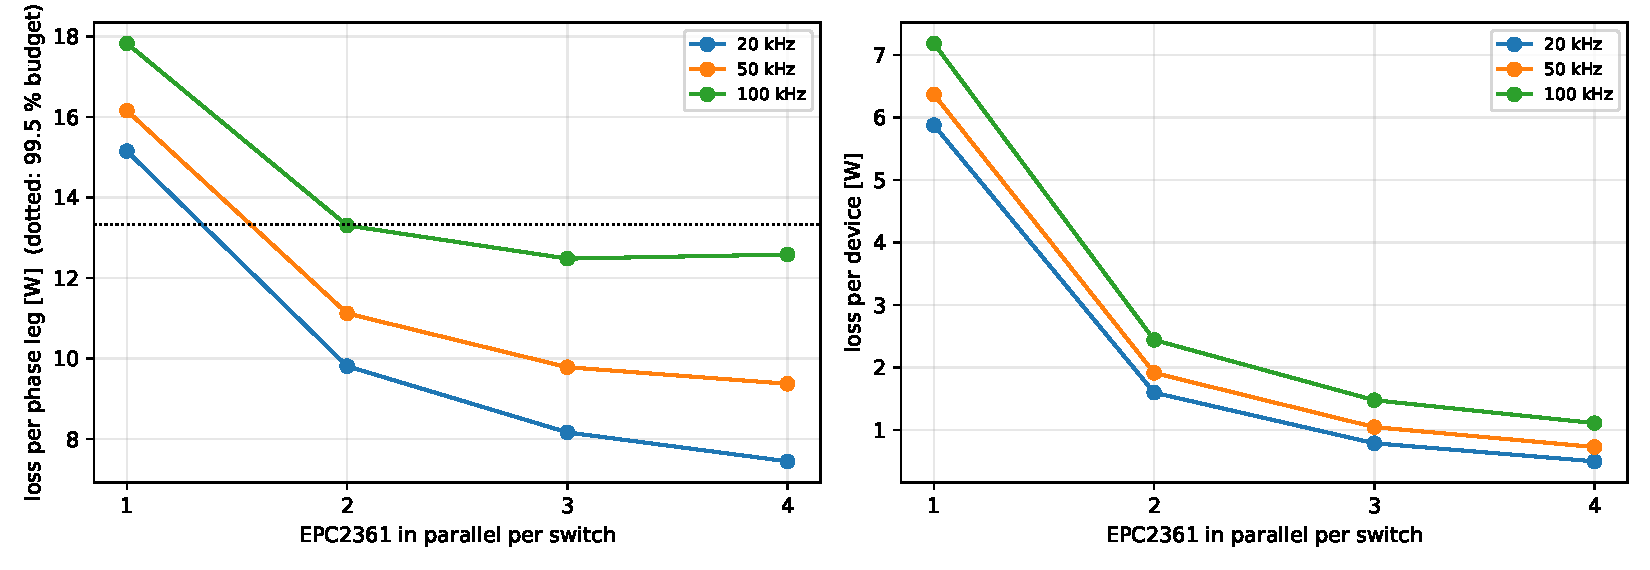
\includegraphics[width=0.85\textwidth]{n_parallel.pdf}
\caption{Loss per leg (left) and per device (right) versus devices per switch. The switching energy is scaled from the $n$\,=\,2 LTspice $E(i)$ fit.}\label{fig:npar}
\end{figure}

%=====================================================================
\section{Loss model and switching-frequency selection}\label{sec:loss}
%=====================================================================
\subsection{Loss model}
Adapting~\cite{zou2025} to a GaN leg with $n$ devices per switch, sinusoidal current and dead time $t_\mathrm{dt}$:
\begin{align}
P_\mathrm{cond}&=\frac{I_\mathrm{rms}^2\,R_\mathrm{DS(on)}(T_j)}{n}, &
P_\mathrm{sw}&=f_\mathrm{sw}\,\frac1\pi\int_0^\pi\!\big[E_\mathrm{on}(i)+E_\mathrm{off}(i)\big]\,d\theta,\quad i=\hat I\sin\theta,\\
P_\mathrm{dt}&=2f_\mathrm{sw}t_\mathrm{dt}\,\overline{\big(V_{SD}(i)\,|i|\big)}, &
P_\mathrm{Cu}&=\sum_h \tfrac12\,\mathbf{I}_h^\mathsf{H}\,\mathbf{R}(f_h)\,\mathbf{I}_h\quad(\text{Q3D sweep}),
\end{align}
plus the gate-drive and MLCC ESR losses. $\mathbf{I}_h$ are the copper branch currents at harmonic $f_h$ of the switched FET currents, obtained from a nodal solve of the board network with the Q3D matrices $\mathbf{R}(f)$, $\mathbf{L}(f)$, the MLCC groups and the DC-supply impedance.
$E_\mathrm{on}(i)$ and $E_\mathrm{off}(i)$ are quadratic fits of LTspice DPT runs with the extracted parasitics and the selected gate resistors, so the layout is inside the loss model.
The $V_\mathrm{SD}$ of the GaN reverse conduction ($\approx$\,2\,V) makes the dead-time term non-negligible. A negative off-voltage would increase it further~\cite{tran2025,wattenberg2023}, which is one reason for the 0\,V off-state used here.

\textbf{Switching-harmonic copper loss.} A Q3D frequency sweep (1\,kHz--100\,MHz) shows that the copper resistance is already about 1.5$\times$ its DC value at 50\,kHz and 3$\times$ at 500\,kHz, because the current crowds onto the facing surfaces and the lowest-inductance paths of the planes. Solving the board network (Q3D $R(f)$, $L(f)$, MLCC groups, DC-supply impedance, switched FET currents for SVM) at every harmonic gives \PcuHf\,W of copper loss at the switching harmonics on top of the \Pcu\,W from the load current, up to \PcuHfLowM\,W at low modulation index where the ripple current is largest. Most of the ripple current comes from the 1210 bank above the cells and crosses the planes; the same network gives \Pcap\,W of MLCC ESR loss.
\begin{figure}[H]\centering
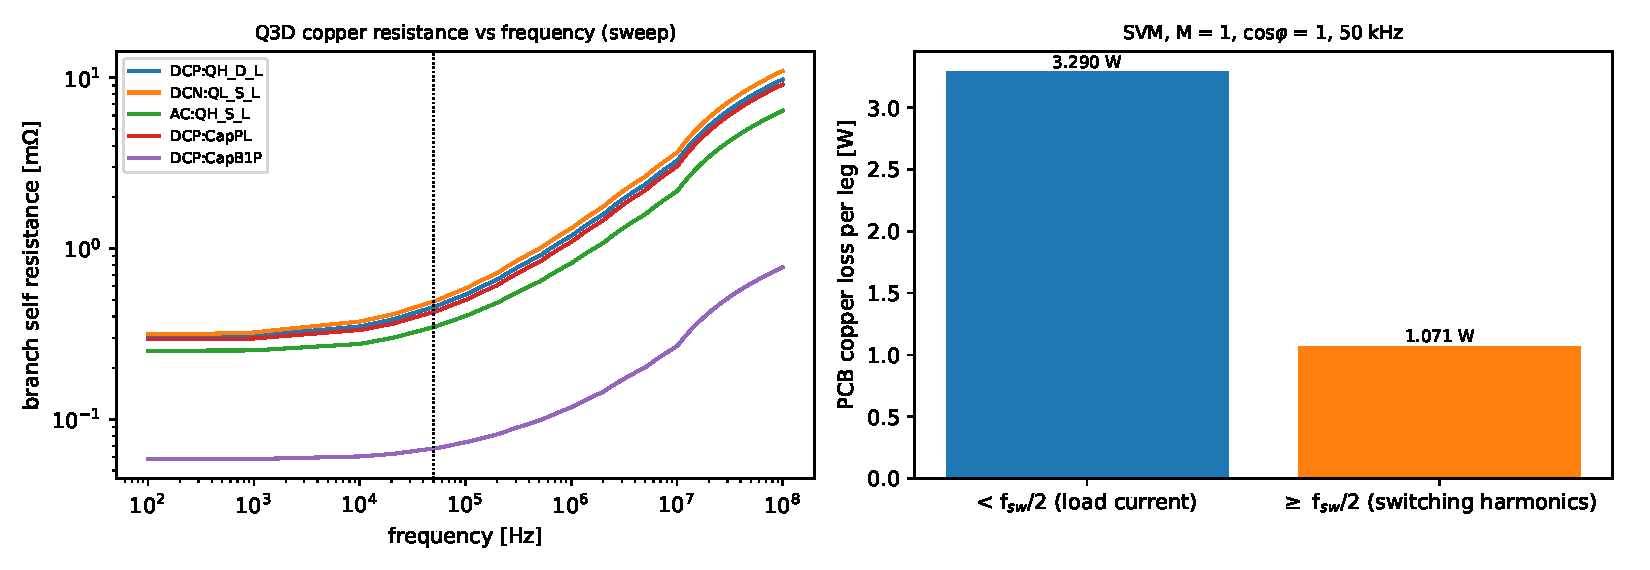
\includegraphics[width=0.95\textwidth]{copper_hf.pdf}
\caption{Left: Q3D copper resistance of the main branches versus frequency. Right: copper loss per leg split into the load-current part and the switching-harmonic part (SVM, $M=1$, $\cos\varphi=1$, 50\,kHz).}\label{fig:cuhf}
\end{figure}
Conduction, switching and dead-time losses are identical for SPWM and SVM at the same current; only the switching-harmonic copper loss differs slightly (0.88\,W for SPWM vs.\ \PcuHf\,W for SVM at $M=1$), and SVM additionally reaches $M=1.15$. The high- and low-side switches share the loss equally: with synchronous GaN conduction $\overline{d\,i^2}=\overline{i^2}/2$ for any $M$ and $\cos\varphi$.

\begin{figure}[H]\centering
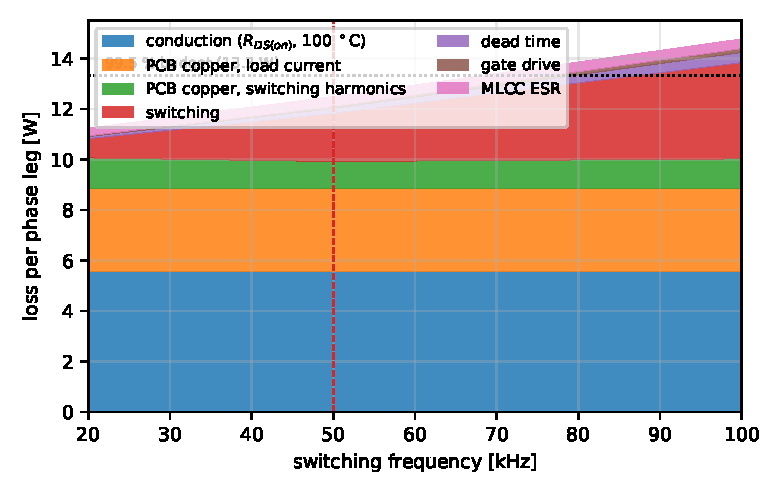
\includegraphics[width=0.62\textwidth]{loss_stack.pdf}
\caption{Loss breakdown per leg. Conduction and PCB copper are about 80\,\% of the loss at 50\,kHz; switching is linear in $f_\mathrm{sw}$, and the 99.5\,\% budget is reached at about 60\,kHz.}\label{fig:loss}
\end{figure}

\subsection{Loss characterisation}
The graphs below follow the datasheet-driven loss study used for the 2\,kV SiC inverter, but with the switching energies taken from LTspice with the Q3D layout parasitics instead of datasheet double-pulse data, so they include the actual loop and gate resistors of this board.

\begin{figure}[H]\centering
\begin{minipage}{0.5\textwidth}\centering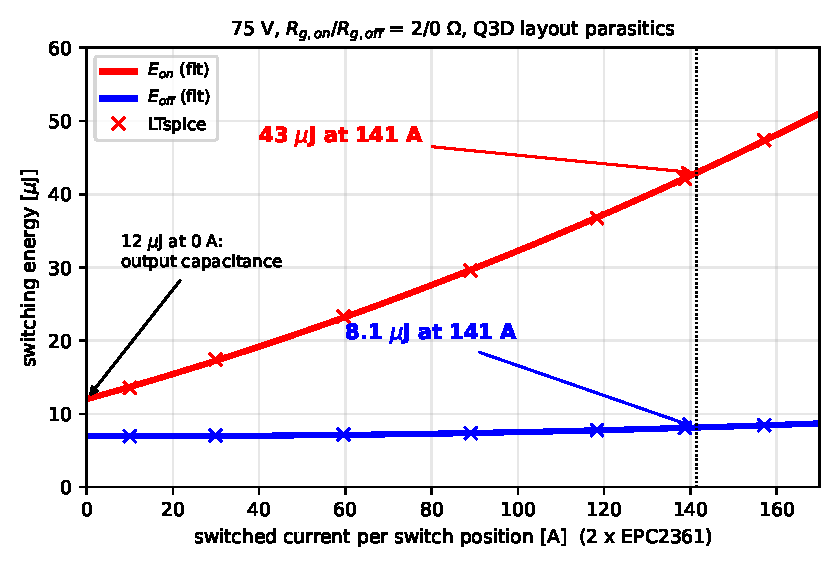
\includegraphics[width=\textwidth]{lc_energy.pdf}\end{minipage}\hfill
\begin{minipage}{0.48\textwidth}\centering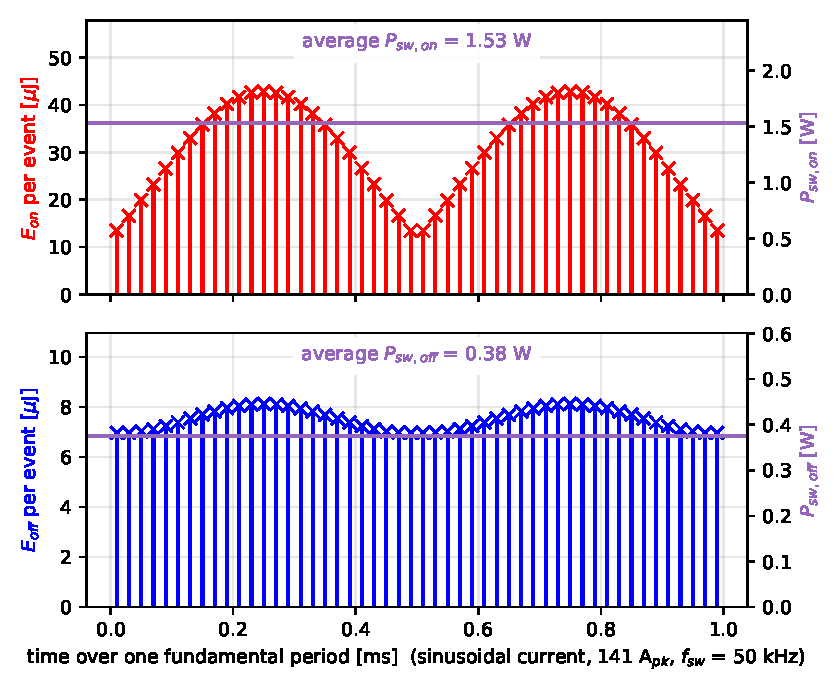
\includegraphics[width=\textwidth]{lc_events.pdf}\end{minipage}
\caption{Left: switching energies of one switch position (2\,$\times$\,EPC2361) versus current: \LcEonPk\,\textmu J ($E_\mathrm{on}$) and \LcEoffPk\,\textmu J ($E_\mathrm{off}$) at the rated peak of \Ipk\,A. Right: energy of each switching event over one fundamental period for a sinusoidal 100\,A$_\mathrm{rms}$ current at 50\,kHz (fundamental 1\,kHz for display); the averages give $P_\mathrm{sw,on}$\,=\,\LcPon\,W and $P_\mathrm{sw,off}$\,=\,\LcPoff\,W. The same result holds for SPWM and SVM, since every leg switches once per period at the instantaneous current.}\label{fig:lcenergy}
\end{figure}

\begin{figure}[H]\centering
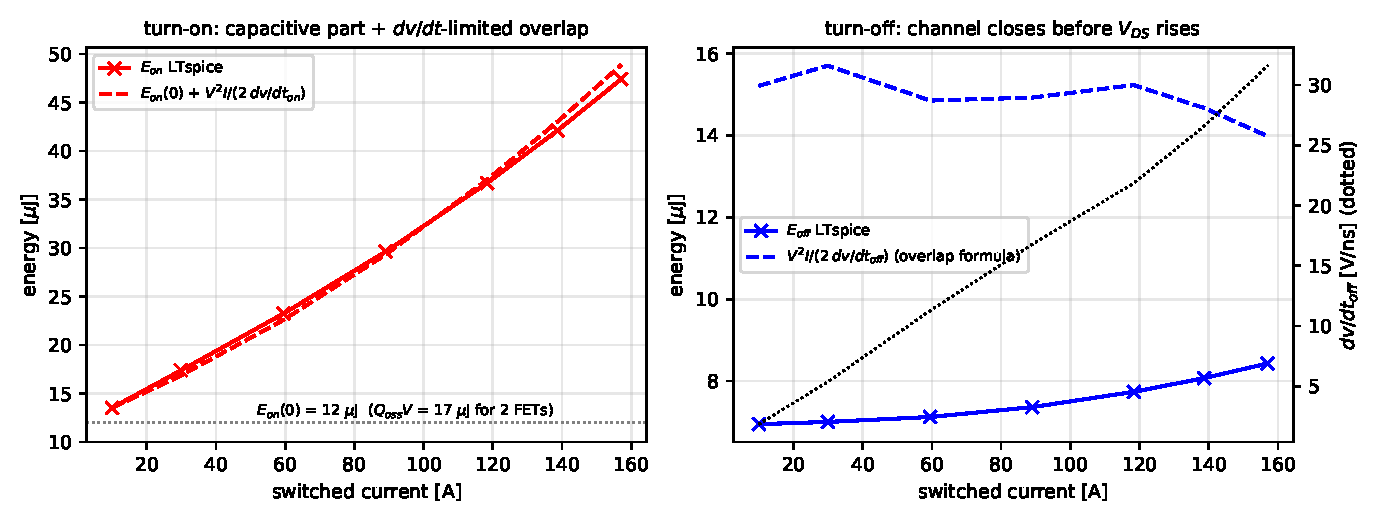
\includegraphics[width=0.95\textwidth]{lc_decomp.pdf}
\caption{Decomposition of the switching energy. Turn-on: a current-independent output-capacitance part ($E_\mathrm{on}(0)$\,=\,\LcEonZeroFit\,\textmu J, of the order of $Q_\mathrm{oss}V$\,=\,\LcQossV\,\textmu J for two FETs) plus an overlap part that follows $V^2I/(2\,dv/dt)$ closely (\LcOvOnPk\ vs.\ \LcEonMinusZeroPk\,\textmu J at \LcIpkMeas\,A, $dv/dt_\mathrm{on}$\,=\,\LcDvOnPk\,V/ns). Turn-off: the classical overlap formula overestimates by about 2$\times$ (\LcOvOffPk\ vs.\ \LcEoffMeasPk\,\textmu J) because the GaN channel closes before $V_\mathrm{DS}$ rises and the load current charges $C_\mathrm{oss}$; $dv/dt_\mathrm{off}$ (dotted) rises with current up to \LcDvOffPk\,V/ns.}\label{fig:lcdecomp}
\end{figure}
Unlike the 2\,kV SiC case, where the output-capacitance energy grows with the number of dies and the overlap loss is limited by the slow datasheet $dv/dt$, here the zero-current part is about one third of $E_\mathrm{on}$ at the rated current and the turn-on overlap is set by the selected $R_\mathrm{g,on}$ (Section~\ref{sec:gate}).

\begin{figure}[H]\centering
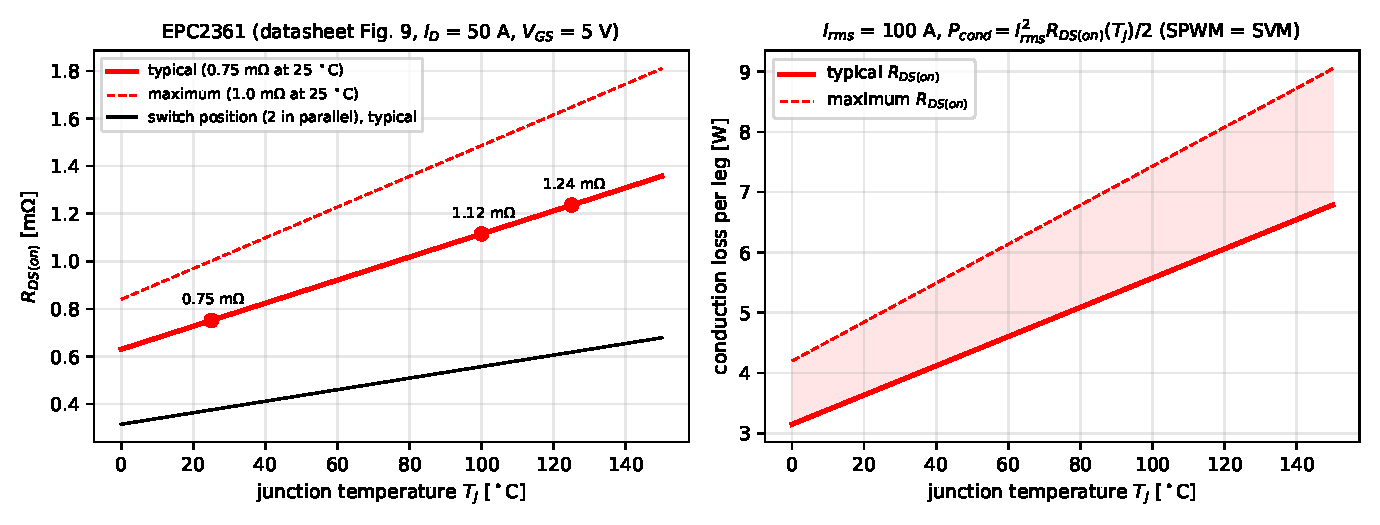
\includegraphics[width=0.95\textwidth]{lc_rds_cond.pdf}
\caption{Left: $R_\mathrm{DS(on)}$ of EPC2361 versus junction temperature (datasheet Fig.~9, linear from 0.84 to 1.81$\times$ the 25\,$^\circ$C value between 0 and 150\,$^\circ$C). Right: conduction loss per leg at 100\,A$_\mathrm{rms}$; identical for SPWM and SVM.}\label{fig:lcrds}
\end{figure}

\begin{figure}[H]\centering
\begin{minipage}{0.55\textwidth}\centering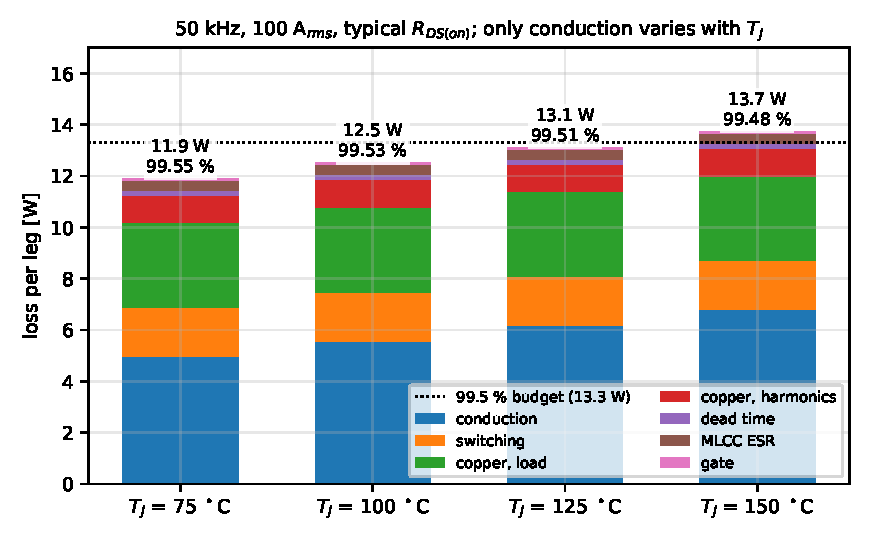
\includegraphics[width=\textwidth]{lc_tj.pdf}\end{minipage}\hfill
\begin{minipage}{0.42\textwidth}\small\centering
\begin{tabular}{@{}lcccc@{}}\toprule
$T_j$ [$^\circ$C] & 75 & 100 & 125 & 150 \\\midrule
$P_\mathrm{cond}$ [W] & \LcCondSeventyFive & \LcCondHundred & \LcCondOneTwentyFive & \LcCondOneFifty \\
Loss [W] & \LcTotSeventyFive & \LcTotHundred & \LcTotOneTwentyFive & \LcTotOneFifty \\
$\eta$ [\%] & \LcEtaSeventyFive & \LcEtaHundred & \LcEtaOneTwentyFive & \LcEtaOneFifty \\
$\eta$, max $R_\mathrm{DS(on)}$ & \LcEtaMaxSeventyFive & \LcEtaMaxHundred & \LcEtaMaxOneTwentyFive & \LcEtaMaxOneFifty \\
\bottomrule\end{tabular}\\[2mm]
\footnotesize As in the 2\,kV study, only the conduction loss is varied with $T_j$; no thermal model is used. In reality $E_\mathrm{on}$ also rises with $T_j$~\cite{zou2025} and the copper resistance rises by about 0.4\,\%/K with the board temperature, so the values at high $T_j$ are optimistic.
\end{minipage}
\caption{Loss and efficiency per leg versus junction temperature at 50\,kHz. With typical devices the 99.5\,\% target holds up to about 130\,$^\circ$C; with maximum $R_\mathrm{DS(on)}$ it is missed above about 67\,$^\circ$C.}\label{fig:lctj}
\end{figure}

\subsection{Slow switching: larger gate resistances}\label{sec:slow}
A motor-friendly design may slow the switching with larger gate resistors, as EPC does on its four-parallel motor-drive board (10\,$\Omega$ on, 2\,$\Omega$ off). Six resistor pairs were simulated with the full building-block model over 10--160\,A (Fig.~\ref{fig:slowE}); energies are integrated from the waveforms over 400\,ns while $V_\mathrm{DS}>1$\,V, so the conduction tail is excluded.

\begin{figure}[H]\centering
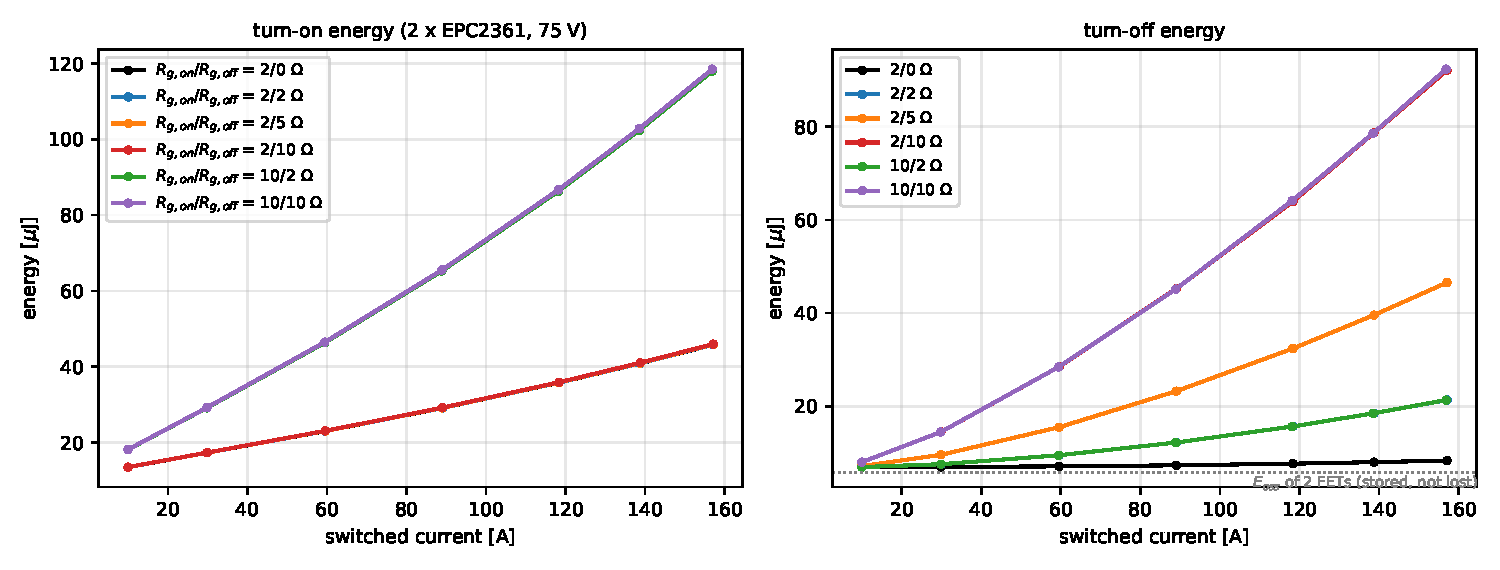
\includegraphics[width=0.92\textwidth]{slow_energy.pdf}
\caption{Switching energies for $R_\mathrm{g,on}/R_\mathrm{g,off}$ pairs. $E_\mathrm{on}$ depends only on $R_\mathrm{g,on}$ and $E_\mathrm{off}$ only on $R_\mathrm{g,off}$, so curves with equal resistor overlap (2/2 and 10/2; 2/10 and 10/10).}\label{fig:slowE}
\end{figure}

\textbf{When is the turn-off channel-controlled?} The voltage rise takes either the time the load current needs to move the output charge, $t_\mathrm{load}=Q_\mathrm{oss,tot}/I$, or the time the gate needs to remove the Miller charge, $t_\mathrm{gate}\approx Q_\mathrm{GD}R_\mathrm{g,off,tot}/V_\mathrm{pl}$. The slower one sets $dv/dt$. Only when the gate is slower does the channel carry current while $V_\mathrm{DS}$ rises, i.e.\ when
\begin{equation}
R_\mathrm{g,off,tot}>R_\mathrm{crit}=\frac{V_\mathrm{pl}\,Q_\mathrm{oss,tot}}{I\,Q_\mathrm{GD}} .
\end{equation}
With $Q_\mathrm{oss,tot}\approx$\,\SlowCoss\,nF\,$\times$\,75\,V (from the load-driven slope in Fig.~\ref{fig:slowF}, right), $Q_\mathrm{GD}$\,=\,3.8\,nC and a plateau of about 2\,V, $R_\mathrm{crit}\approx$\,1.5\,$\Omega$ at 139\,A and 7\,$\Omega$ at 30\,A. This matches the simulations: the selected 0.8\,$\Omega$ total stays load-driven at every current; 2.8\,$\Omega$ (2\,$\Omega$ external) becomes gate-driven above about 50\,A; 10.8\,$\Omega$ is gate-driven almost everywhere.

\begin{figure}[H]\centering
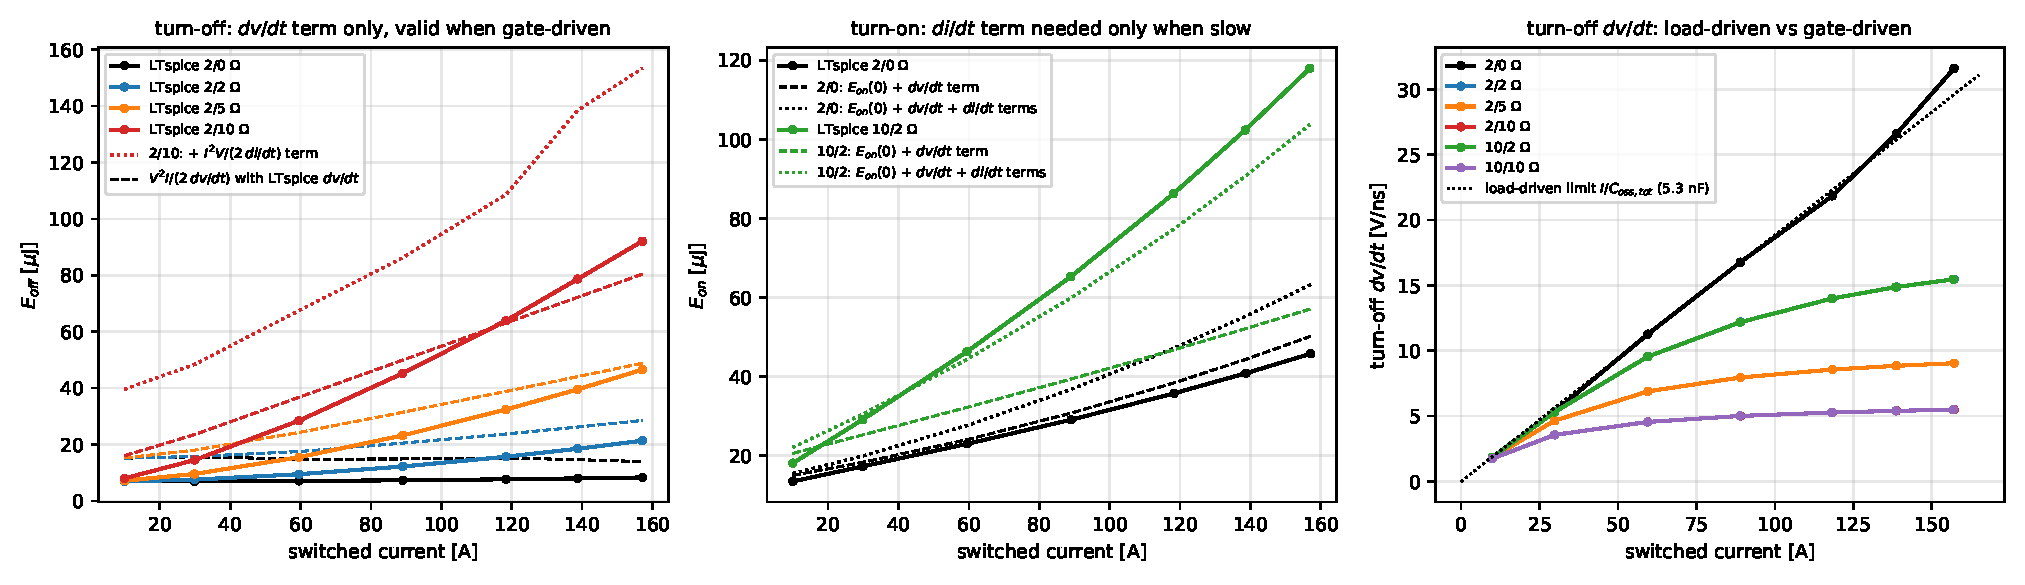
\includegraphics[width=\textwidth]{slow_formula.pdf}
\caption{Left: $E_\mathrm{off}$ (solid) against $V^2I/(2\,dv/dt)$ with the simulated $dv/dt$ (dashed); the dotted curve adds the $I^2V/(2\,di/dt)$ term for 2/10\,$\Omega$. Centre: $E_\mathrm{on}$ against $E_\mathrm{on}(0)$ plus the overlap terms. Right: turn-off $dv/dt$; the dotted line is the load-driven limit $I/C_\mathrm{oss,tot}$.}\label{fig:slowF}
\end{figure}

\textbf{Is the overlap formula valid?}
\begin{itemize}\itemsep1pt
\item \emph{Turn-off, gate-driven} ($R_\mathrm{g,off,tot}>R_\mathrm{crit}$): yes, with the $dv/dt$ term only, $E_\mathrm{off}\approx V^2I/(2\,dv/dt)$, within about 10\,\% (2/10\,$\Omega$: 50/63/72\,\textmu J against 45/64/79\,\textmu J at 89/118/139\,A). Adding the $I^2V/(2\,di/dt)$ term overestimates by about 1.8$\times$: the simulation shows no separate loss in the current-fall phase.
\item \emph{Turn-off, load-driven} ($R_\mathrm{g,off,tot}<R_\mathrm{crit}$, the selected design): no. The formula gives about 15\,\textmu J at any current, the simulation 7--8\,\textmu J, of which 5.8\,\textmu J is $E_\mathrm{oss}$ stored in the two FETs.
\item \emph{Turn-on, fast} (2\,$\Omega$): $E_\mathrm{on}\approx E_\mathrm{on}(0)+V^2I/(2\,dv/dt)$; the $di/dt$ term is not needed.
\item \emph{Turn-on, slow} (10\,$\Omega$): both terms are needed, $E_\mathrm{on}\approx E_\mathrm{on}(0)+V^2I/(2\,dv/dt)+I^2V/(2\,di/dt)$, within about 10\,\%, because the current rise becomes a separate slow phase ($di/dt$ 65$\to$19\,A/ns at 139\,A).
\end{itemize}

\begin{table}[H]\centering\footnotesize
\caption{Slow-switching cases at 139\,A (LTspice) and loss at the rated point, 50\,kHz (all other losses unchanged).}\label{tab:slow}
\setlength{\tabcolsep}{4pt}
\begin{tabular}{@{}lcccccccc@{}}\toprule
$R_\mathrm{g,on}/R_\mathrm{g,off}$ [$\Omega$] & $E_\mathrm{on}$ [\textmu J] & $E_\mathrm{off}$ [\textmu J] & $dv/dt_\mathrm{on}$ & $dv/dt_\mathrm{off}$ [V/ns] & peak $V_\mathrm{DS}$ [V] & HS bump [V] & $P_\mathrm{sw}$ [W] & $\eta$ [\%] \\\midrule
2/0 (selected) & \SlEonBase & \SlEoffBase & \SlDvOnBase & \SlDvOffBase & \SlVdsBase & \SlBumpBase & \SlPswBase & \SlEtaBase \\
2/2 & \SlEonOffTwo & \SlEoffOffTwo & \SlDvOnOffTwo & \SlDvOffOffTwo & \SlVdsOffTwo & \SlBumpOffTwo & \SlPswOffTwo & \SlEtaOffTwo \\
2/5 & \SlEonOffFive & \SlEoffOffFive & \SlDvOnOffFive & \SlDvOffOffFive & \SlVdsOffFive & \SlBumpOffFive & \SlPswOffFive & \SlEtaOffFive \\
2/10 & \SlEonOffTen & \SlEoffOffTen & \SlDvOnOffTen & \SlDvOffOffTen & \SlVdsOffTen & \SlBumpOffTen & \SlPswOffTen & \SlEtaOffTen \\
10/2 (EPC motor board) & \SlEonOnTen & \SlEoffOnTen & \SlDvOnOnTen & \SlDvOffOnTen & \SlVdsOnTen & \SlBumpOnTen & \SlPswOnTen & \SlEtaOnTen \\
10/10 & \SlEonBoth & \SlEoffBoth & \SlDvOnBoth & \SlDvOffBoth & \SlVdsBoth & \SlBumpBoth & \SlPswBoth & \SlEtaBoth \\
\bottomrule\end{tabular}\end{table}
Observations:
\begin{itemize}\itemsep1pt
\item $R_\mathrm{g,off}$ is the effective knob for the turn-off $dv/dt$ only above $R_\mathrm{crit}$; 10\,$\Omega$ brings it from 27 to 5\,V/ns at 139\,A, at a cost of about 70\,\textmu J per event.
\item $R_\mathrm{g,on}$\,=\,10\,$\Omega$ mainly slows $di/dt$; the turn-on $dv/dt$ only falls from about 13 to 11\,V/ns, while $E_\mathrm{on}$ rises 2.5$\times$. It does reduce the high-side overshoot (peak $V_\mathrm{DS}$ of QH 83.5$\to$74.7\,V).
\item The same $R_\mathrm{g,off}$ also holds the complementary FET off: its gate bump rises from 0.99 to 1.29\,V with $R_\mathrm{g,off}$, above $V_\mathrm{th,typ}$. Slowing the turn-off therefore needs a separate low-impedance hold-off path (Miller clamp) or a negative off-voltage.
\item The fully slow 10/10\,$\Omega$ design costs about 4\,W of switching loss per leg at 50\,kHz and misses the 99.5\,\% target (\SlEtaBoth\,\%). The selected 2/0\,$\Omega$ is the efficient choice; if the machine requires a lower $dv/dt$, a moderate $R_\mathrm{g,off}$ with a Miller clamp is the cheaper lever.
\end{itemize}
($P_\mathrm{sw}$ of the 2/0 case here is \SlPswBase\,W instead of \Psw\,W because the conduction tail inside the original 150\,ns window is excluded.)

\subsection{Why a high switching frequency}
Cooke and Rogers show a visible reduction of the phase-current ripple from 20 to 50\,kHz with a GaN inverter~\cite{cooke2026}, and Wattenberg et al.\ use the higher frequency to replace electrolytic capacitors with MLCCs~\cite{wattenberg2023}.
Here the DC-link capacitance halves from 50 to 100\,kHz (Section~\ref{sec:dclink}) at a cost of about 0.44\,W per 10\,kHz in switching loss.

\textbf{Winding ripple requirement.} The machine is not yet defined, so machine-side PWM losses are not evaluated here. The inverter side can, however, state what it requires: the peak-to-peak ripple of a phase is at most $\Delta i_\mathrm{pp}\approx V_\mathrm{dc}/(4L f_\mathrm{sw})$, where $L$ is the inductance seen by the ripple. For $\Delta i_\mathrm{pp}\leq10$\,\% of the 141\,A peak this means $L\geq$\,\LreqTwentyFive, \LreqFifty{} and \LreqHundred\,\textmu H at 25, 50 and 100\,kHz, a requirement to be handed to the machine design.

50\,kHz is chosen as the nominal point; the block stays within the efficiency target up to about \Fmax\,kHz, and the final value is fixed once the machine is selected.

%=====================================================================
\section{Power-loop design}\label{sec:loop}
%=====================================================================
\subsection{Analytical estimate and dominant parameters}
For a vertical loop with forward and return currents on adjacent layers, the partial-inductance estimate used in~\cite{cooke2026,tran2025} is
\begin{equation}
L_\mathrm{loop}\approx\mu_0\,\frac{h\,l}{w},
\end{equation}
with dielectric thickness $h$, path length $l$ and width $w$.
For one cell ($l\approx10$\,mm, $w$\,=\,9\,mm) this gives \KanNHmm\,nH per mm of dielectric, i.e.\ \LanCell\,nH at $h$\,=\,0.1\,mm.
Q3D gives a slope of \KqNHmm\,nH/mm, close to the analytical value. Q3D also shows a fixed part of \LfixNH\,nH (vias, device pads and package) that no dielectric reduction can remove (Fig.~\ref{fig:loopvh}).
Table~\ref{tab:loopparams} lists the geometric parameters, following the parameter table of~\cite{tran2025}.

\begin{figure}[H]\centering
\begin{minipage}{0.47\textwidth}\centering
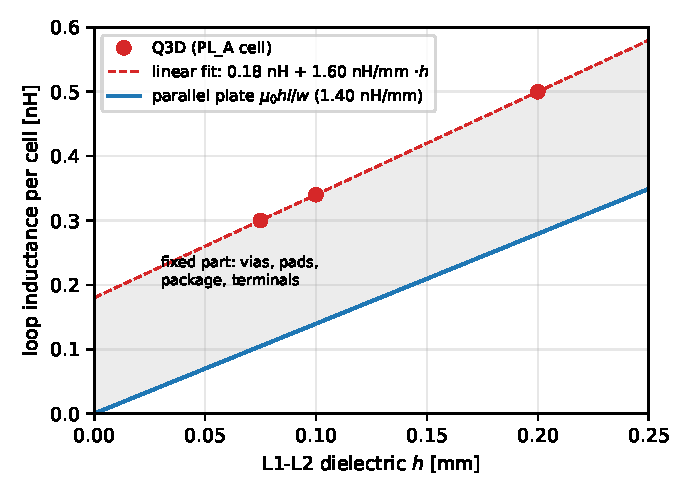
\includegraphics[width=\textwidth]{loop_vs_h.pdf}
\captionof{figure}{Loop inductance per cell versus the L1--L2 dielectric: analytical slope versus Q3D.}\label{fig:loopvh}
\end{minipage}\hfill
\begin{minipage}{0.50\textwidth}\footnotesize
\captionof{table}{Geometric parameters, constraints and choices.}\label{tab:loopparams}
\setlength{\tabcolsep}{3pt}\begin{tabular}{@{}L{1.7cm}L{2.1cm}L{2.2cm}L{2.0cm}@{}}\toprule
Parameter & Effect & Constraint & Choice \\\midrule
$h$ (L1--L2) & $L\propto h$ & 2 plies, $\geq$\,0.075\,mm & 0.1\,mm \\
$l$ (cap$\to$QL S) & $L\propto l$ & 0805 + 2 FET pads & $\approx$\,10\,mm \\
$w$ (cell width) & $L\propto1/w$ & board width & 9\,mm \\
via pitch & fixed part & drill rules & 0.9\,mm \\
local caps & ESL/$N$ & cell length & 6\,$\times$\,0805 \\
copper L2--L4 & $R_\mathrm{Cu}$ & cost, etching & 2\,oz \\
\bottomrule\end{tabular}
\end{minipage}
\end{figure}

\subsection{Layout and extraction}
The block uses mirrored cells at $x=\pm7.5$\,mm. Each cell has its own vertical loop: the high-side drain row and six 0805 capacitors on L1, and the return on the DC$-$ plane on L2, 0.1\,mm below.
The bulk MLCC rows above the cells feed both cells symmetrically. This follows the distributed-bank recommendation of~\cite{brothers2019}, which avoids the cascaded, shared loop inductance that caused the 2\,MHz resonance of the commercial module.
\begin{figure}[H]\centering
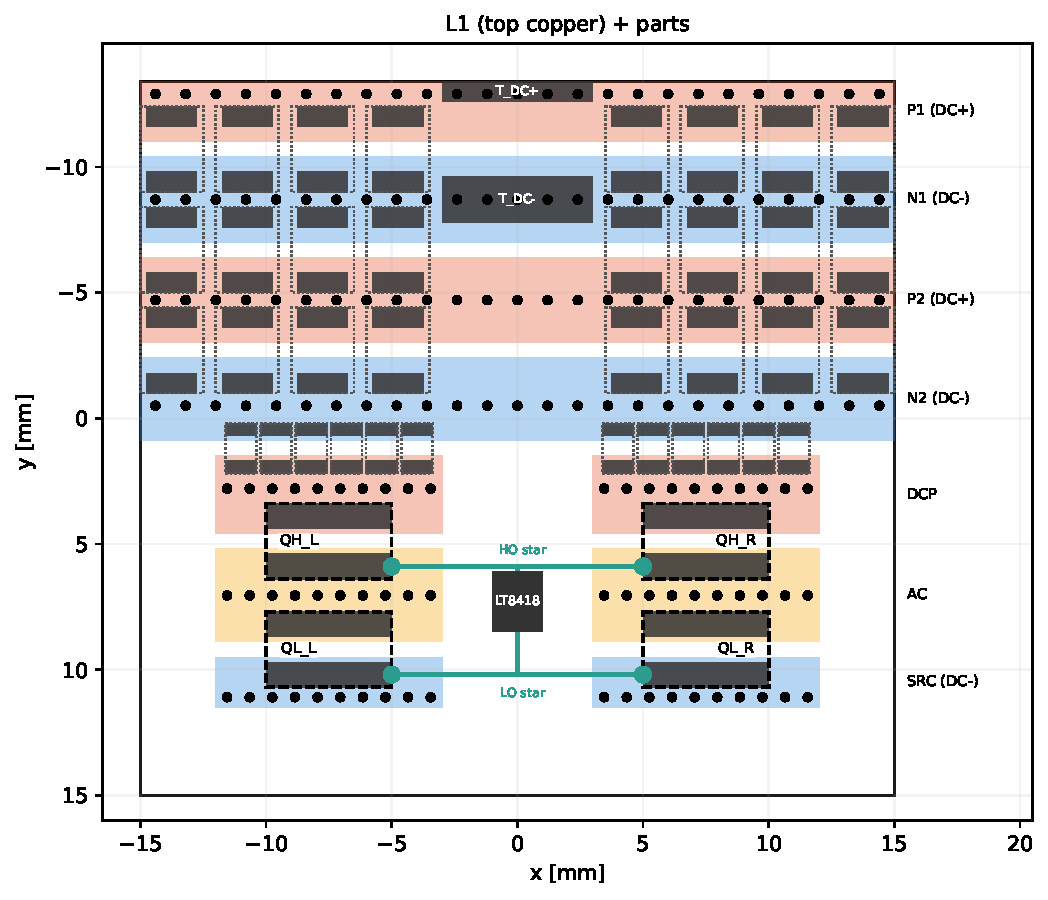
\includegraphics[width=0.60\textwidth]{layout_top.pdf}\hfill
\begin{minipage}[b]{0.37\textwidth}\centering
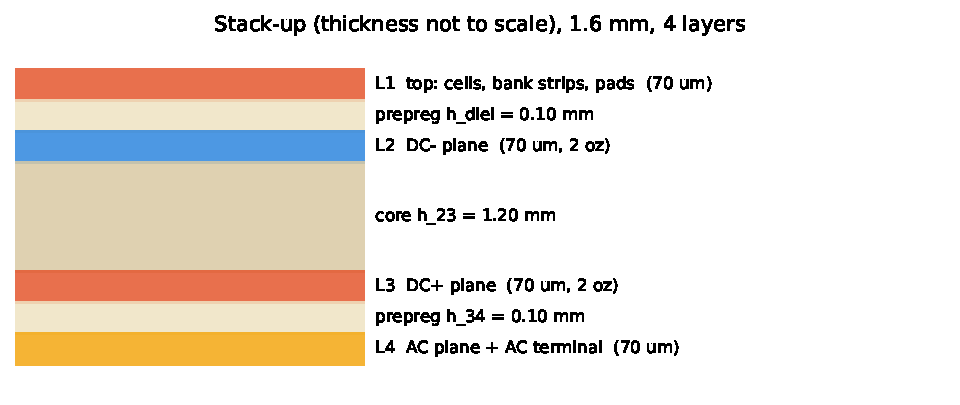
\includegraphics[width=\textwidth]{layout_stackup.pdf}\\[2mm]
\small L1 cells and bank, L2 DC$-$, L3 DC+, L4 AC; 2\,oz copper.
\end{minipage}
\caption{Layout generated from the same geometry as the Q3D model.}
\end{figure}
Q3D extracts the partial $R/L$ matrix of the copper with every component as a gap between source and sink terminals.
As in~\cite{tran2025}, the loop inductance follows from the matrix.
For a branch-wise description, $L_\mathrm{loop}=L_D+L_S+L_\mathrm{ac}+2(M_{DS}-M_{D,ac}-M_{S,ac})$.
Here the full 21-terminal matrix is instead exported to LTspice as coupled inductors (\texttt{K} elements), and the effective loop is obtained by a nodal solve with both cells excited.
The result is \LloopCu\,nH copper and \LloopEsl\,nH with MLCC ESL per cell.
Each FET sees this cell loop; paralleling halves the current and $di/dt$ per loop, not the inductance. The EPC2361 package inductance and post-routing details are not included, so the measured loop will be somewhat higher.

\subsection{Overshoot design space}
\begin{figure}[H]\centering
\begin{minipage}{0.52\textwidth}\centering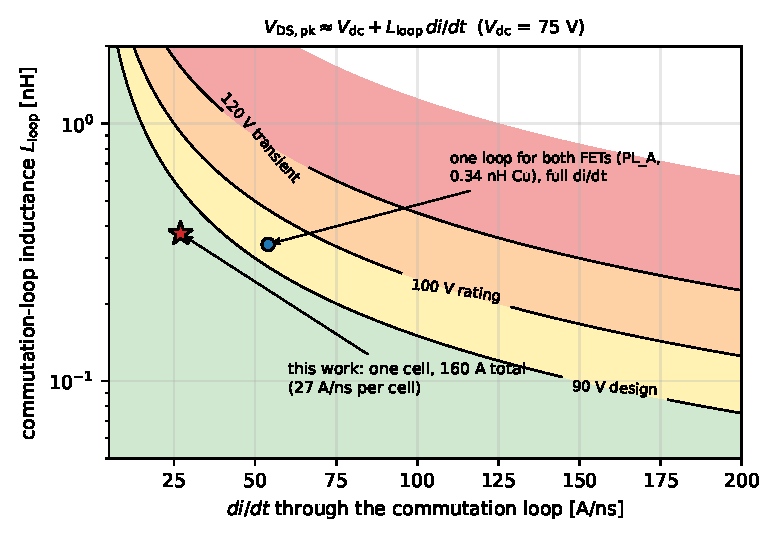
\includegraphics[width=\textwidth]{overshoot_map.pdf}\end{minipage}\hfill
\begin{minipage}{0.45\textwidth}
\captionof{figure}{First-order overshoot map $V_\mathrm{DS,pk}=V_\mathrm{dc}+L_\mathrm{loop}\,di/dt$. The operating point uses the effective $di/dt$ through one cell (\DidtCell\,A/ns) that reproduces the LTspice peak at 160\,A. At this $di/dt$ the 90\,V design limit allows $L_\mathrm{loop}\leq$\,\LloopMaxNine\,nH per cell, which leaves room for the package and routing additions. A single loop carrying both FETs (PL\_A) sees the full $di/dt$ and would be at the 100\,V rating.}\label{fig:ovs}
\end{minipage}
\end{figure}

%=====================================================================
\section{Gate-drive design}\label{sec:gate}
%=====================================================================
\subsection{Mechanisms}
Tran et al.\ write the gate voltage of paralleled devices during $di/dt$ and $dv/dt$ as~\cite{tran2025}
\begin{align}
v_{gs,j}&=v_\mathrm{drv}-i_{g,j}(R_{g,j}+R_{s,j})-(L_{g,j}+L_{sg,j})\frac{di_{g,j}}{dt}-M_{gs,j}\frac{di_{D,j}}{dt}-L_{sg,j}\frac{d\Delta i_D}{dt}, \\
v_{gs,j}&\approx v_\mathrm{drv,off}+C_{gd}\frac{dv_{DS}}{dt}(R_{g}+R_{s})+(L_{g}+L_{sg})\,C_{gd}\frac{d^2v_{DS}}{dt^2}\quad\text{(turn-off of the complementary switch)}.
\end{align}
The first equation shows why mismatched quasi-common-source inductance (which drives a circulating current $\Delta i_D$) and power-to-gate coupling $M_{gs}$ are the dominant risks for paralleled devices.
The second gives the Miller bump. Fig.~\ref{fig:parmap} maps every parasitic to its effect and to the layout rule adopted in this design.

\begin{figure}[H]\centering
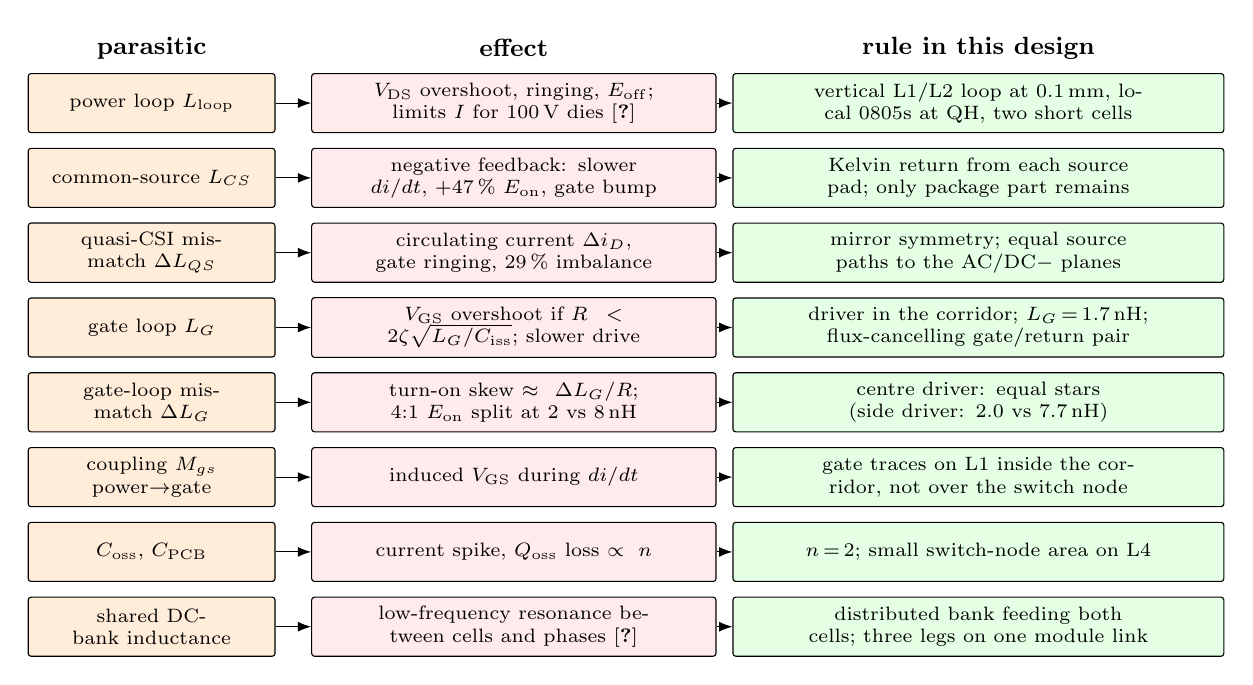
\begin{tikzpicture}[font=\scriptsize,node distance=1.2mm]
\tikzset{p/.style={draw,fill=orange!15,rounded corners=1pt,text width=2.9cm,minimum height=0.75cm,align=center},
         e/.style={draw,fill=red!8,rounded corners=1pt,text width=4.9cm,minimum height=0.75cm,align=center},
         r/.style={draw,fill=green!10,rounded corners=1pt,text width=6.0cm,minimum height=0.75cm,align=center}}
\node[font=\small\bfseries] at (0,0.7) {parasitic};
\node[font=\small\bfseries] at (4.6,0.7) {effect};
\node[font=\small\bfseries] at (10.5,0.7) {rule in this design};
\foreach \i/\a/\b/\c in {
 0/{power loop $L_\mathrm{loop}$}/{$V_\mathrm{DS}$ overshoot, ringing, $E_\mathrm{off}$; limits $I$ for 100\,V dies~\cite{brothers2019}}/{vertical L1/L2 loop at 0.1\,mm, local 0805s at QH, two short cells},
 1/{common-source $L_{CS}$}/{negative feedback: slower $di/dt$, +47\,\% $E_\mathrm{on}$, gate bump}/{Kelvin return from each source pad; only package part remains},
 2/{quasi-CSI mismatch $\Delta L_{QS}$}/{circulating current $\Delta i_D$, gate ringing, 29\,\% imbalance}/{mirror symmetry; equal source paths to the AC/DC$-$ planes},
 3/{gate loop $L_G$}/{$V_\mathrm{GS}$ overshoot if $R<2\zeta\sqrt{L_G/C_\mathrm{iss}}$; slower drive}/{driver in the corridor; $L_G$\,=\,1.7\,nH; flux-cancelling gate/return pair},
 4/{gate-loop mismatch $\Delta L_G$}/{turn-on skew $\approx\Delta L_G/R$; 4:1 $E_\mathrm{on}$ split at 2 vs 8\,nH}/{centre driver: equal stars (side driver: 2.0 vs 7.7\,nH)},
 5/{coupling $M_{gs}$ power$\to$gate}/{induced $V_\mathrm{GS}$ during $di/dt$}/{gate traces on L1 inside the corridor, not over the switch node},
 6/{$C_\mathrm{oss}$, $C_\mathrm{PCB}$}/{current spike, $Q_\mathrm{oss}$ loss $\propto n$}/{$n$\,=\,2; small switch-node area on L4},
 7/{shared DC-bank inductance}/{low-frequency resonance between cells and phases~\cite{brothers2019}}/{distributed bank feeding both cells; three legs on one module link}}
{
 \node[p] (p\i) at (0,-\i*0.95) {\a};
 \node[e] (e\i) at (4.6,-\i*0.95) {\b};
 \node[r] (r\i) at (10.5,-\i*0.95) {\c};
 \draw[-{Latex}] (p\i)--(e\i); \draw[-{Latex}] (e\i)--(r\i);
}
\end{tikzpicture}
\caption{Parasitic--effect--rule map (after~\cite{lu2017,tran2025}). Percentages are from the 2\,$\times$\,EPC2361 sensitivity study (Section~\ref{sec:sharing}).}\label{fig:parmap}
\end{figure}

\subsection{Gate-resistor design window}
Treating the gate loop as a series RLC with $C_\mathrm{iss}$ gives a lower bound for the turn-on resistance (no $V_\mathrm{GS}$ overshoot)~\cite{tran2025,lu2017,musumeci2022}.
The Miller current through the turn-off path gives an upper bound for the turn-off resistance:
\begin{equation}
R_{G,\mathrm{on,tot}}\geq2\zeta\sqrt{\frac{L_G}{C_\mathrm{iss}}}\;(\zeta=0.707:\ \RdampMin\,\Omega),\qquad
R_{G,\mathrm{off,tot}}\leq\frac{V_\mathrm{th}}{C_\mathrm{rss}\,dv/dt}\;(\RoffMaxMin\text{--}\RoffMaxTyp\,\Omega\ \text{at}\ \DvdtOff\,\mathrm{V/ns}).
\end{equation}
The selected totals are \RonTot\,$\Omega$ on ($R_g$\,+\,$R_{G,\mathrm{int}}$\,+\,driver pull-up, $\zeta$\,=\,\ZetaOn) and \RoffTot\,$\Omega$ off ($R_{G,\mathrm{int}}$ plus the shared pull-down, $\zeta$\,=\,\ZetaOff). Both are inside the window (Fig.~\ref{fig:rgw}).
Within the window, the turn-on value is set by the LTspice sweep (Fig.~\ref{fig:rgstudy}).
Below 2\,$\Omega$ the high-side overshoot exceeds 90\,V (112\,V at 0.5\,$\Omega$). Above it, $E_\mathrm{on}$ grows.
$R_\mathrm{g,off}$ hardly changes $E_\mathrm{off}$ because the turn-off is load-driven: the channel closes before $V_\mathrm{DS}$ rises and the load current charges $C_\mathrm{oss}$ ($dv/dt\approx I/2C_\mathrm{oss,tot}$).
$R_\mathrm{g,off}$ therefore only weakens hold-off, and 0\,$\Omega$ is chosen.

\begin{figure}[H]\centering
\begin{minipage}{0.49\textwidth}\centering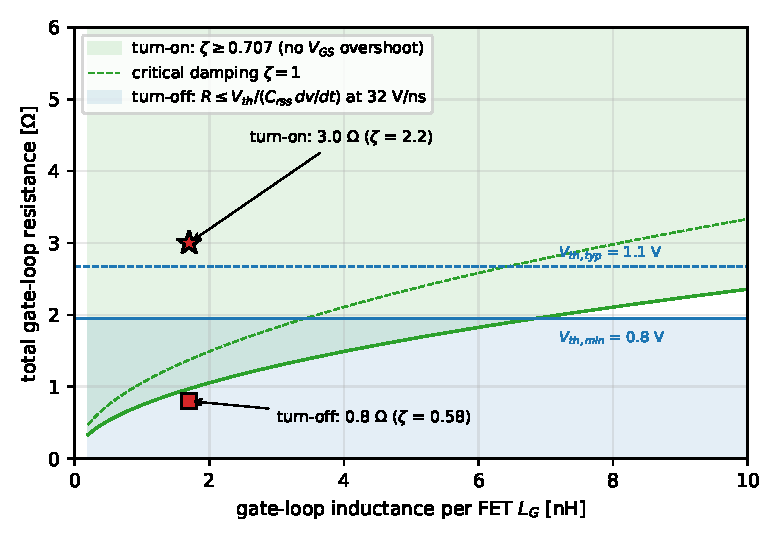
\includegraphics[width=\textwidth]{rg_window.pdf}
\captionof{figure}{Gate-resistor design window for EPC2361 ($C_\mathrm{iss}$\,=\,3.6\,nF, $C_\mathrm{rss}$\,=\,13\,pF).}\label{fig:rgw}\end{minipage}\hfill
\begin{minipage}{0.49\textwidth}\centering\small
\captionof{table}{Driver comparison (datasheet values).}
\begin{tabular}{@{}L{2.2cm}L{1.0cm}L{1.5cm}L{1.6cm}@{}}\toprule
Driver & Rating & Src/sink & Verdict \\\midrule
LMG1210 & 200\,V & 1.5/3\,A & too weak \\
uP1966E & 85\,V & 0.7/0.4\,$\Omega$ & 5\,V margin \\
LT8418 & 100\,V & 4/8\,A & baseline \\
2EDL5014AA & 120\,V & 4/4\,A & alternative \\
\bottomrule\end{tabular}\\[2mm]
\footnotesize Requirements: bootstrap clamp ($V_\mathrm{SW}$ goes 2--3\,V negative in dead time~\cite{wattenberg2023}), split outputs, CMTI $\geq$\,100\,V/ns, one driver per switch (no driver-to-driver delay skew~\cite{tran2025}).
\end{minipage}
\end{figure}

\begin{figure}[H]\centering
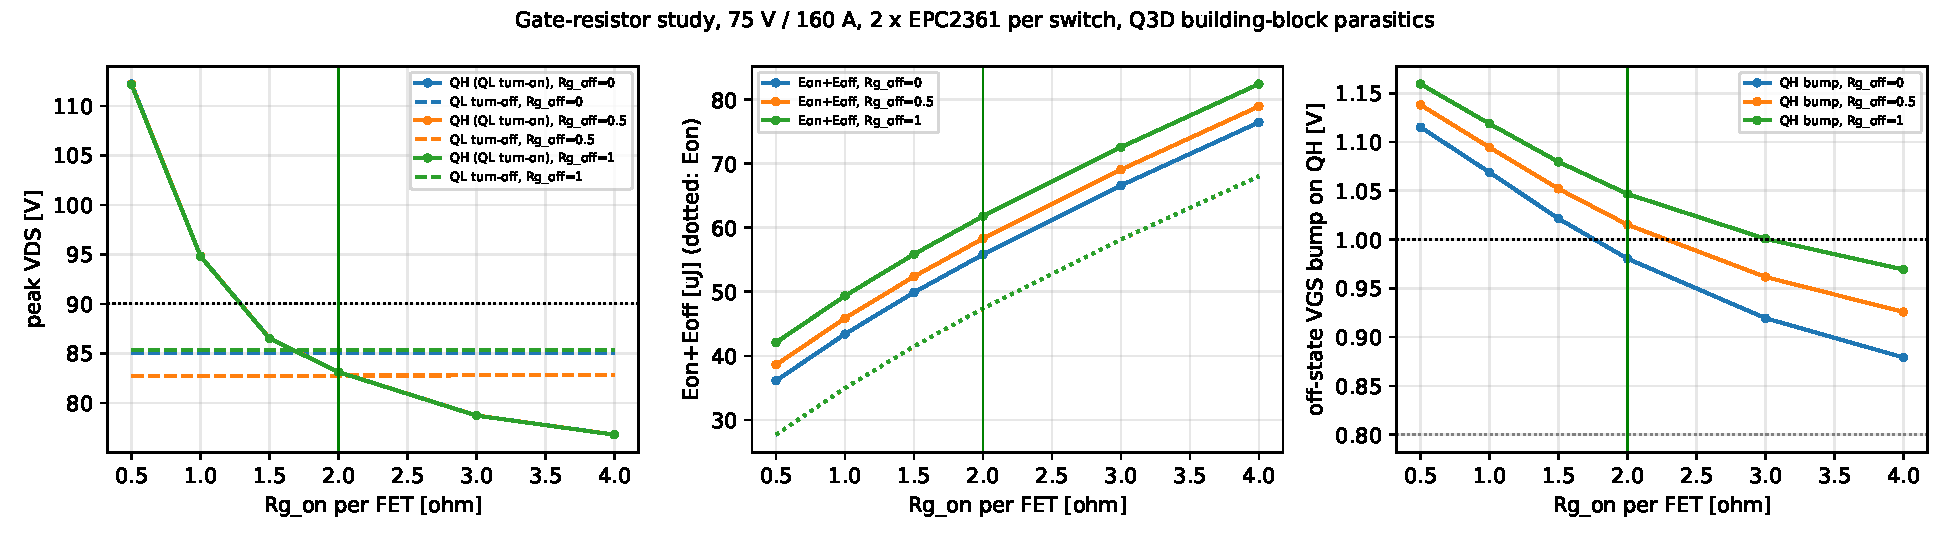
\includegraphics[width=0.95\textwidth]{rg_study.pdf}
\caption{LTspice $R_g$ study at 160\,A with the Q3D parasitics. Selected: \RgOn/\RgOff\,$\Omega$, giving QH \VdsH\,V, QL \VdsL\,V and a gate bump of \VgsBump\,V.}\label{fig:rgstudy}
\end{figure}

\textbf{Gate-bump margin (open risk).} The simple Miller estimate gives \VbumpMiller\,V. The LTspice bump is \VgsBump\,V, which includes common-source and $L_G\,C_{gd}\,d^2v/dt^2$ terms.
This is \UtilBump\,\% of $V_\mathrm{th,typ}$ and above $V_\mathrm{th,min}$ (0.8\,V), so a low-threshold part could partially turn on for a few ns.
The literature offers four mitigations:
\begin{itemize}\itemsep0pt
\item an external $C_\mathrm{GS}$ (270\,pF in~\cite{wattenberg2023}), at some cost in speed;
\item a small negative off-voltage ($-1.5$\,V in~\cite{wattenberg2023}, $-3$\,V in~\cite{tran2025,cooke2026}), at the cost of dead-time loss and a bootstrap level shift;
\item an active Miller clamp;
\item a lower $L_{CS}$.
\end{itemize}
These should be evaluated in the next iteration and checked in the DPT.

%=====================================================================
\section{Current sharing}\label{sec:sharing}
%=====================================================================
Following~\cite{musumeci2022,palma2024}, a minimal two-FET LTspice model was perturbed one parameter at a time (Fig.~\ref{fig:tornado}).
The ranking agrees with~\cite{tran2025,lu2017}.
Common-source mismatch without Kelvin returns and gate-loop mismatch dominate. $V_\mathrm{th}$ spread comes next. A drain-path mismatch is benign.
The gate-loop case explains the centre driver. A mismatch delays one gate by about $\Delta L_G/R_\mathrm{tot}$, roughly 2\,ns, which is half the 4\,ns current transition.
On the building block itself, the two FETs carry 78.53 and 78.63\,A at turn-off (Fig.~\ref{fig:wave}).
\begin{figure}[H]\centering
\begin{minipage}{0.52\textwidth}\centering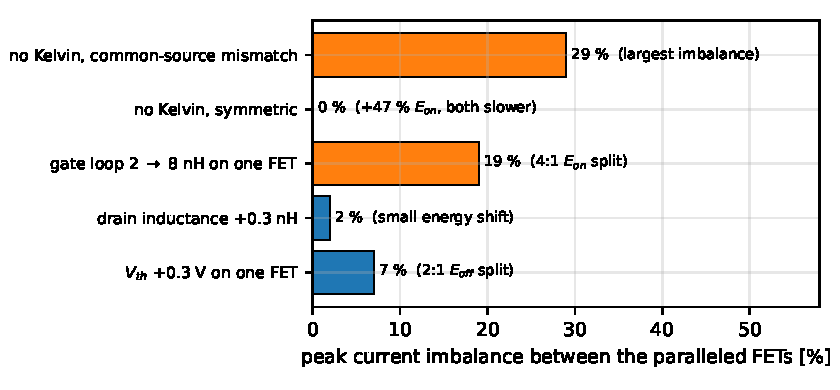
\includegraphics[width=\textwidth]{sharing_tornado.pdf}
\captionof{figure}{Sensitivity of the dynamic current imbalance (75\,V, 120\,A, 2\,$\times$\,EPC2361).}\label{fig:tornado}\end{minipage}\hfill
\begin{minipage}{0.45\textwidth}\centering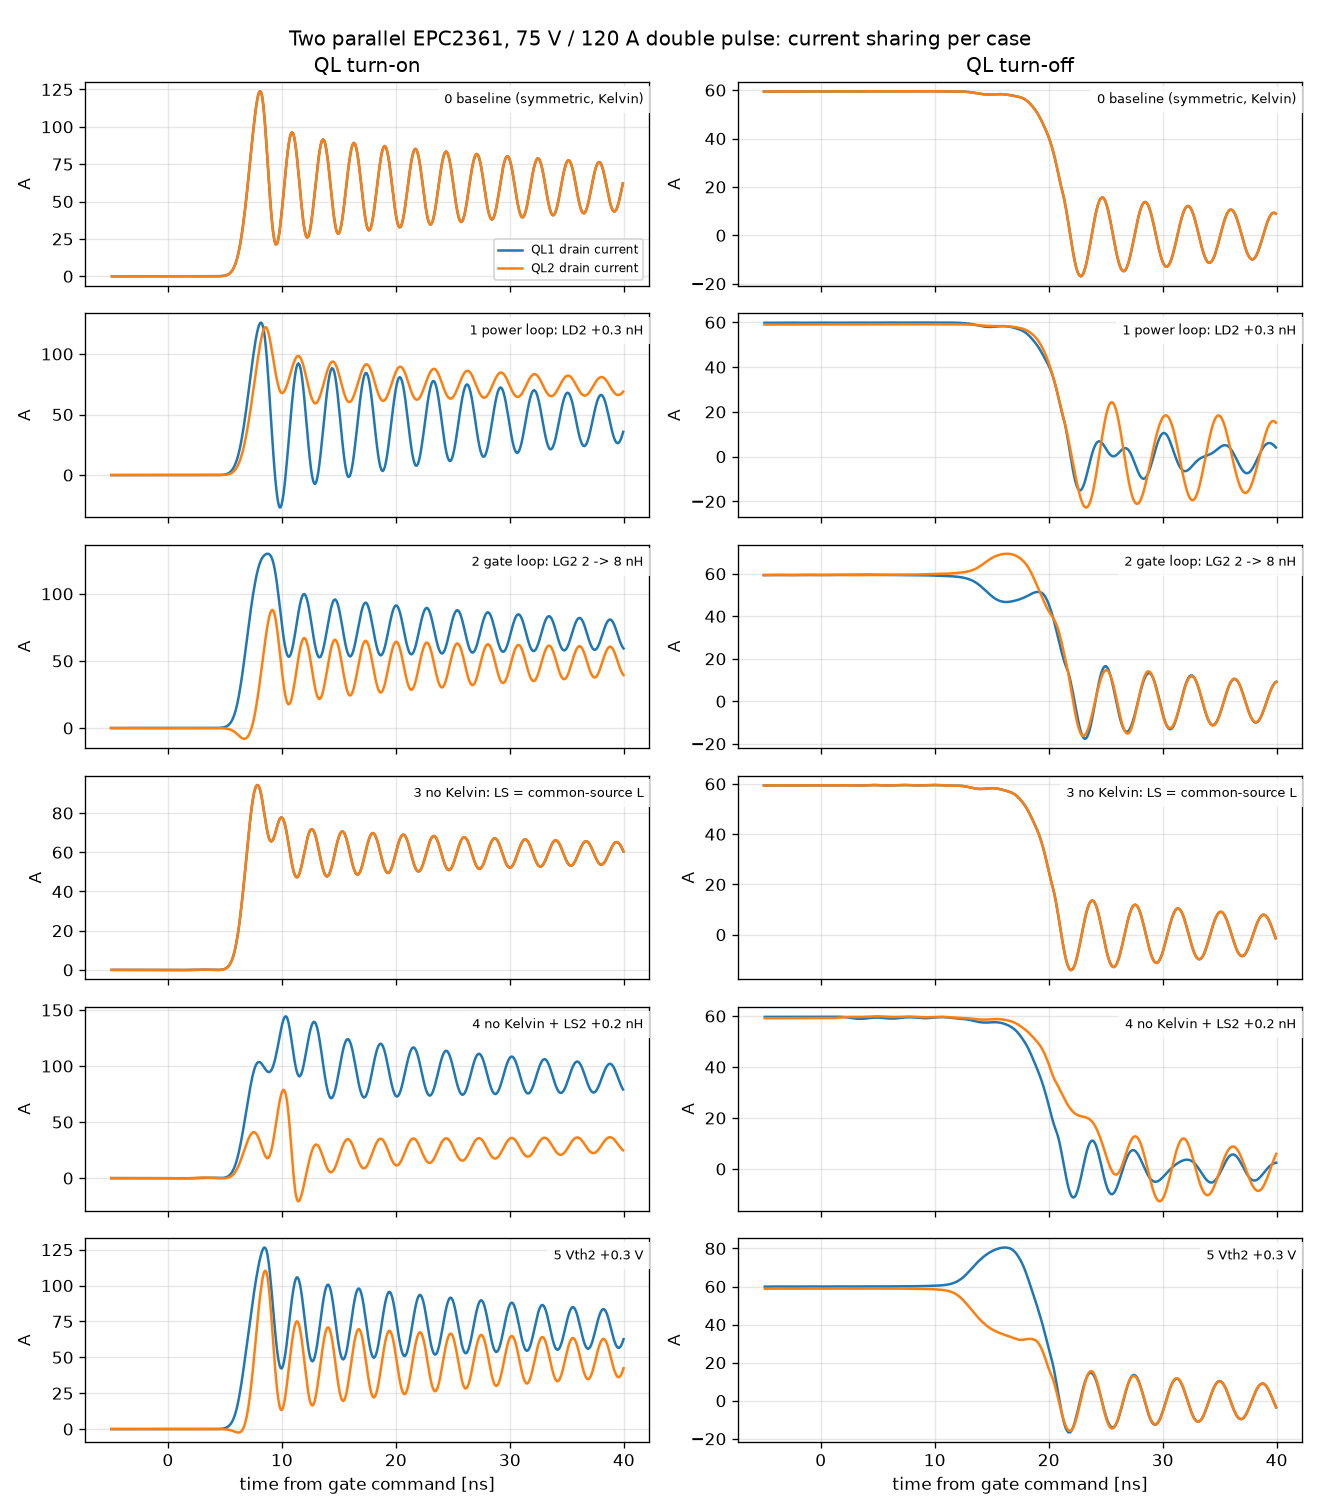
\includegraphics[width=\textwidth]{Sharing_2xEPC2361.png}
\captionof{figure}{Waveforms of the six cases.}\end{minipage}
\end{figure}
\begin{figure}[H]\centering
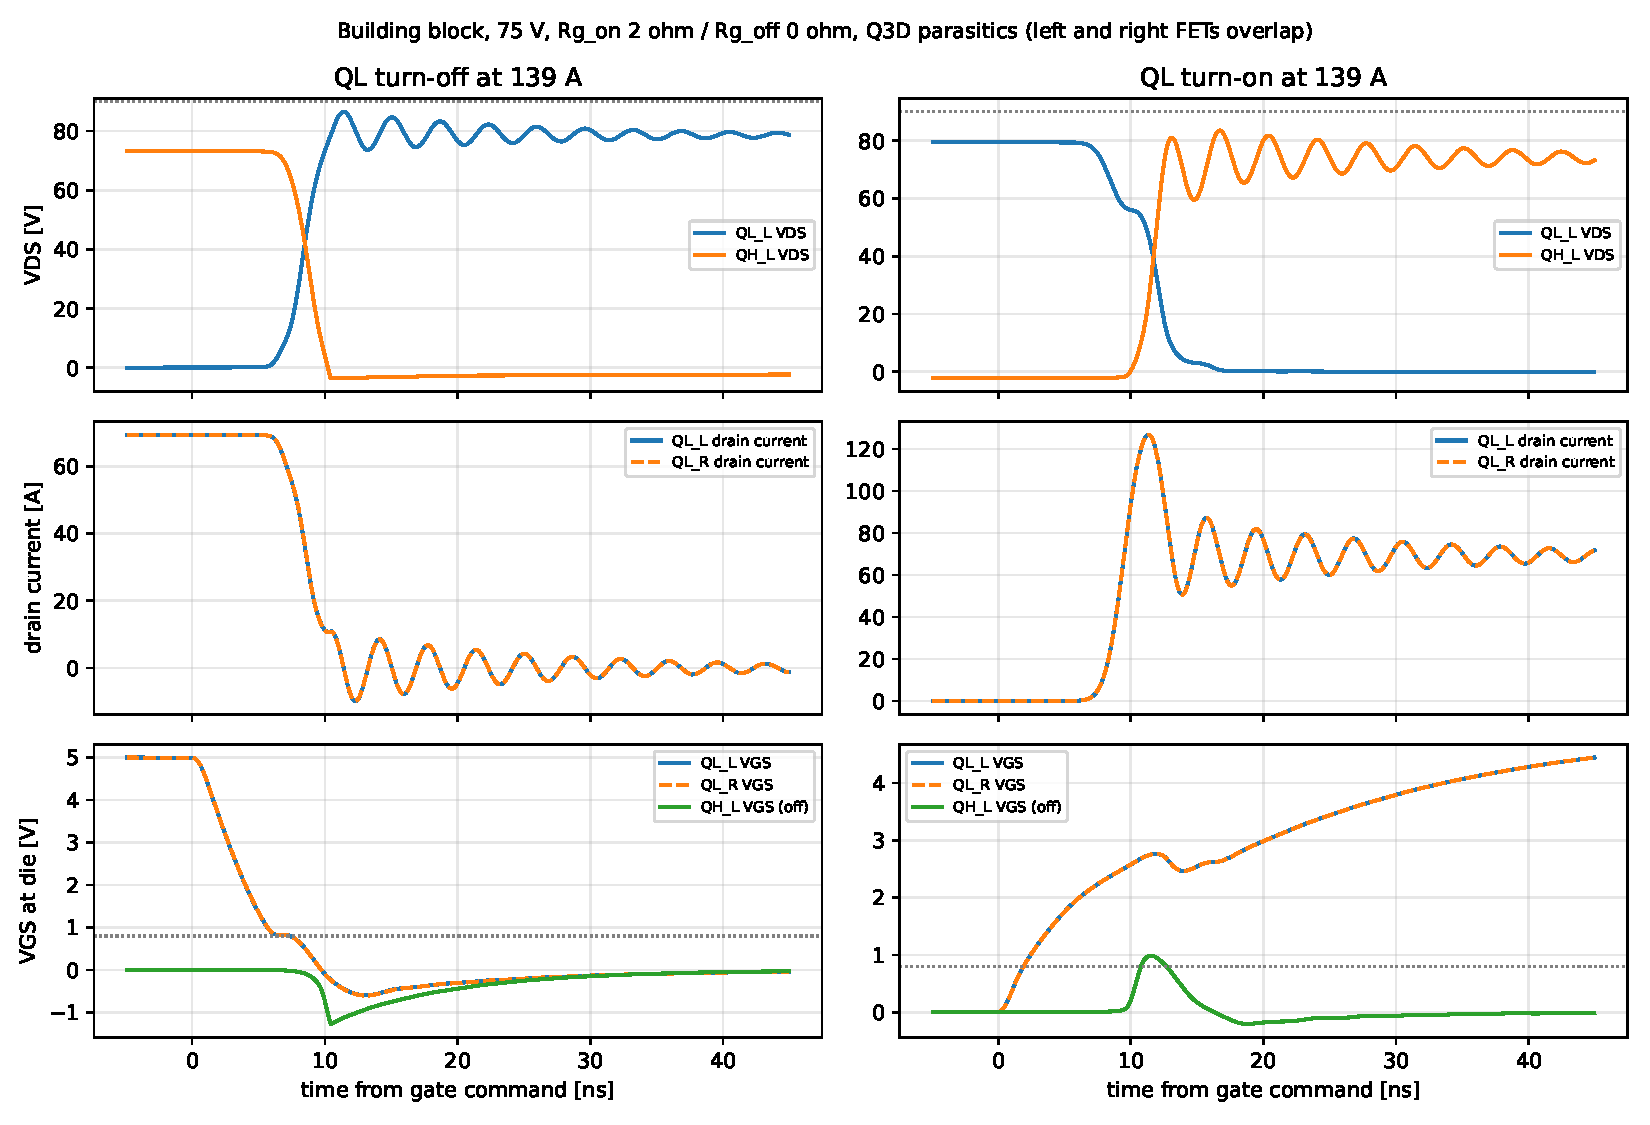
\includegraphics[width=0.85\textwidth]{waveforms_141A.pdf}
\caption{Building-block switching at the rated peak current. The left and right FET currents overlap.}\label{fig:wave}
\end{figure}

%=====================================================================
\section{DC-link design}\label{sec:dclink}
%=====================================================================
As in~\cite{zou2025}, the capacitance is the larger of a voltage-ripple bound and a ripple-current bound, $C_\mathrm{dc}=\max(C_v,C_i)$.
With MLCCs, $C_i$ is a count of parts rather than a capacitance: the HF ripple current (\IlegHFrated\,A$_\mathrm{rms}$ per leg at the rated point, up to \IlegHFworst\,A) divided by the current rating of one capacitor (assumed \Icap\,A, to be confirmed with the manufacturer's data).
$C_v\approx\hat I/(4f_\mathrm{sw}\Delta V_\mathrm{pp})$~\cite{wattenberg2023} is evaluated for three legs on a shared module link (\CreqBlock\,\uF{} per leg at $\pm$2\,\%, 50\,kHz).
Below about \Fcross\,kHz the bank is voltage-limited and shrinks as $1/f_\mathrm{sw}$. Above that it is current-limited and stops shrinking (Fig.~\ref{fig:dcl}). This gives a natural upper bound on the useful $f_\mathrm{sw}$ for density.
MLCC DC-bias derating is included (30\,\% of nominal at 75\,V for the 1210 parts).
\begin{figure}[H]\centering
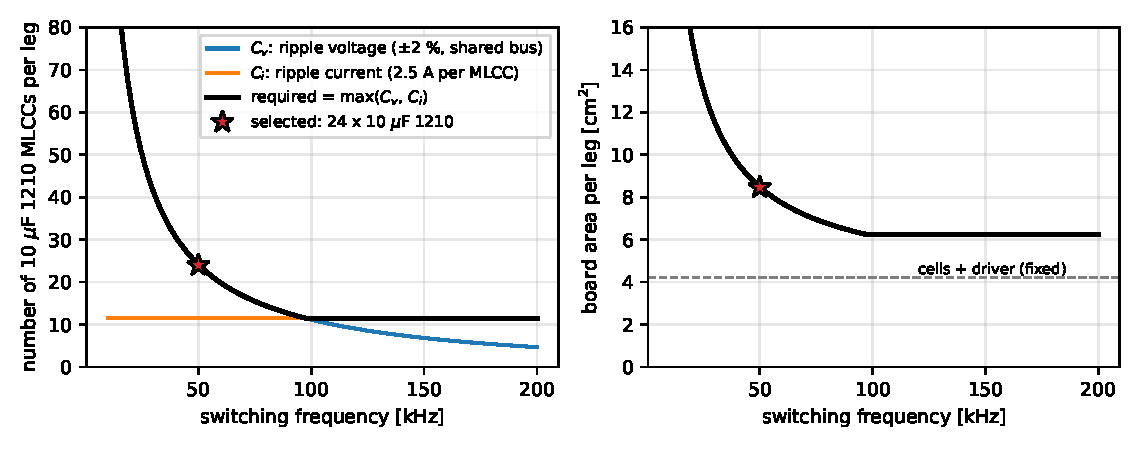
\includegraphics[width=0.92\textwidth]{dclink_space.pdf}
\caption{DC-link design space: MLCC count per leg (left) and resulting board area (right) versus $f_\mathrm{sw}$.}\label{fig:dcl}
\end{figure}
\textbf{DPT bulk capacitance.} During the first pulse the bank must supply the load-inductor energy. Following~\cite{tran2025}:
\begin{equation}
C_\mathrm{DPT}\geq\frac{L_\mathrm{DPT}I_L^2}{2V_\mathrm{dc}\Delta V-\Delta V^2}.
\end{equation}
For $L_\mathrm{DPT}$\,=\,5\,\textmu H and 160\,A ($t_1$\,=\,\Tone\,\textmu s) this requires \CdptTwo\,\uF{} for 2\,\% droop and \CdptFive\,\uF{} for 5\,\%.
The on-board \CeffBlock\,\uF{} is therefore not enough for the DPT, and an external low-inductance film or electrolytic bank of about 0.5--0.6\,mF is needed.

%=====================================================================
\section{Thermal design}\label{sec:thermal}
%=====================================================================
\begin{figure}[H]\centering
\begin{minipage}{0.47\textwidth}\centering
\begin{circuitikz}[scale=0.8,transform shape,font=\small]
\draw (0,0) node[ground]{} to[I,l=$P_\mathrm{dev}$] (0,3) -- (1,3) node[above]{$T_j$}
      to[R,l=$R_\mathrm{\theta JC}$\,0.2] (3,3) node[above]{$T_c$}
      to[R,l=$R_\mathrm{TIM}$\,\Rtim] (5.4,3) node[above]{$T_\mathrm{hs}$}
      to[R,l=$R_\mathrm{hs\text{-}a}$] (5.4,0) node[ground]{};
\draw (1,3) to[R,l=$R_\mathrm{\theta JB}$\,1.5,*-] (1,0.8) -- (2.6,0.8) node[right,font=\scriptsize,align=left]{PCB copper\\(10--15\,\% path~\cite{novo2024})};
\node[font=\scriptsize] at (2.8,4.0) {$\times$4 devices per leg in parallel to $T_\mathrm{hs}$};
\end{circuitikz}
\captionof{figure}{Thermal network per device.}\label{fig:thnet}
\end{minipage}\hfill
\begin{minipage}{0.50\textwidth}\centering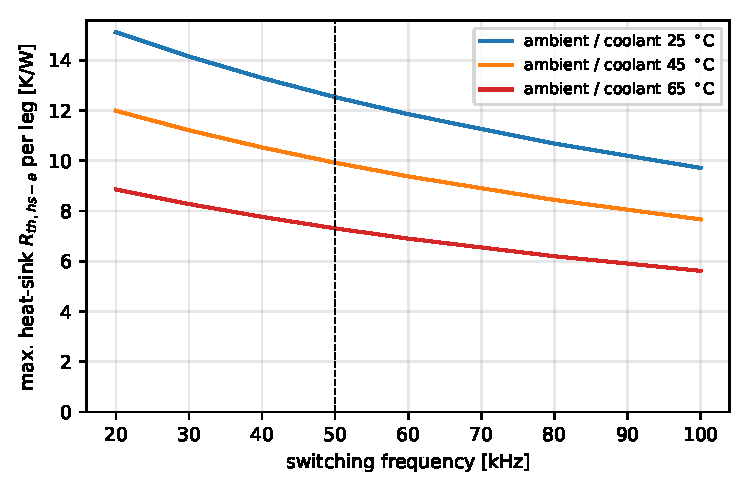
\includegraphics[width=\textwidth]{thermal_req.pdf}
\captionof{figure}{Maximum heat-sink resistance per leg for $T_j\leq$\,125\,$^\circ$C.}\label{fig:threq}\end{minipage}
\end{figure}
Using the constraint of~\cite{zou2025}, $R_\mathrm{hs}\leq\big(T_{j,\max}-T_a-P_\mathrm{dev}(R_\mathrm{\theta JC}+R_\mathrm{TIM})\big)/\sum P_\mathrm{dev}$, the leg needs $R_\mathrm{hs\text{-}a}\leq$\,\RthHsFifty\,K/W with 65\,$^\circ$C coolant at 50\,kHz (\RthHsFiftyCool\,K/W at 45\,$^\circ$C).
This is a mild requirement: with 0.5--1.9\,W per device, a shared cold plate or a small forced-air heat sink suffices.
The TIM, not the heat sink, dominates the per-device rise. For comparison, Cooke and Rogers measured a mean 16.9\,K/W junction-to-ambient per HEMT on a 0.9\,K/W heat sink with 8 devices per switch~\cite{cooke2026}.
The PCB copper loss (\PcuTot\,W) is dissipated mainly in the board and must be included in the board temperature budget.

%=====================================================================
\section{Efficiency--density--frequency co-optimisation}\label{sec:coopt}
%=====================================================================
Zou et al.\ map efficiency and power density over $(f_\mathrm{sw},P_o)$ and select the knee of the Pareto frontier~\cite{zou2025}.
The same is done here at board level, with the area model of Section~\ref{sec:dclink} and the loss model of Section~\ref{sec:loss} (Fig.~\ref{fig:etarho}).
\begin{itemize}\itemsep1pt
\item Raising $f_\mathrm{sw}$ trades efficiency for density until about \Fcross\,kHz (\RhoHundred\,kW/cm$^2$, \EtaHundred\,\% at 100\,kHz). Beyond that the DC link is current-limited, so density no longer improves and only efficiency falls. The frontier therefore ends at about 100\,kHz.
\item 50\,kHz keeps 0.03\,\% efficiency margin at \RhoFifty\,kW/cm$^2$; machine-side losses, which favour higher $f_\mathrm{sw}$, are not included because the machine is not yet defined.
\end{itemize}
\begin{figure}[H]\centering
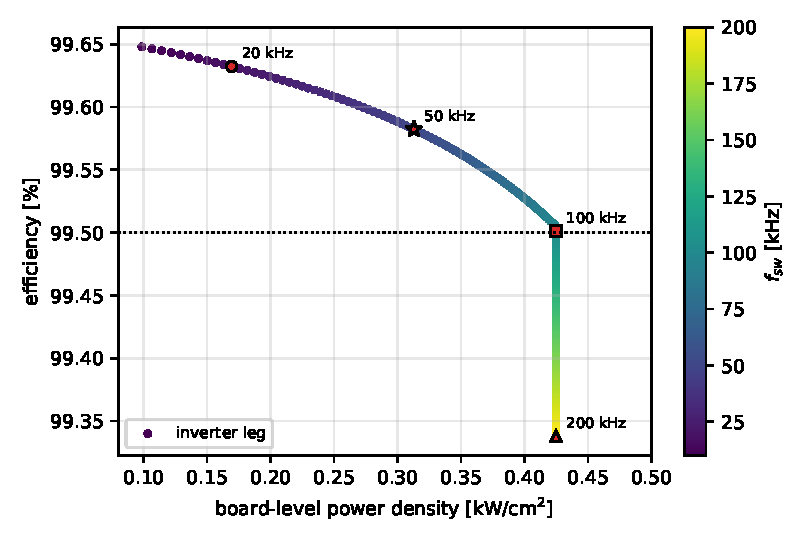
\includegraphics[width=0.62\textwidth]{eta_rho.pdf}
\caption{Efficiency versus board-level power density with $f_\mathrm{sw}$ as the parameter (10--200\,kHz), inverter leg only.}\label{fig:etarho}
\end{figure}

%=====================================================================
\section{Design summary and margins}\label{sec:summary}
%=====================================================================
\begin{figure}[H]\centering
\begin{minipage}{0.45\textwidth}\centering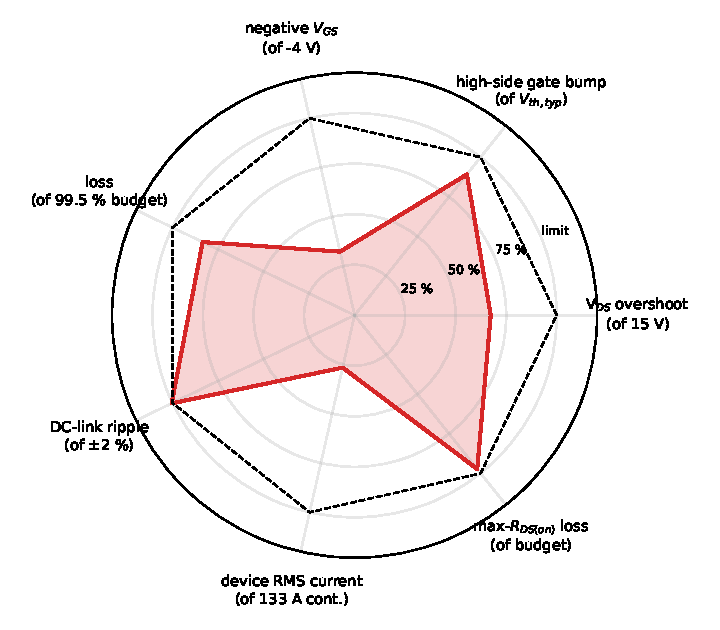
\includegraphics[width=\textwidth]{margins.pdf}
\captionof{figure}{Utilisation of each constraint (1\,=\,limit).}\label{fig:margins}\end{minipage}\hfill
\begin{minipage}{0.52\textwidth}\small
The radar (Fig.~\ref{fig:margins}) shows where the design is tight:
\begin{itemize}\itemsep1pt
\item DC-link ripple at \UtilRipple\,\% of the $\pm$2\,\% target (shared three-leg bus);
\item loss with maximum $R_\mathrm{DS(on)}$ at \UtilWorst\,\% of the budget, i.e.\ above it;
\item high-side gate bump at \UtilBump\,\% of $V_\mathrm{th,typ}$.
\end{itemize}
The voltage overshoot (\UtilVds\,\% of the 15\,V allowance), the negative gate excursion and the device current have comfortable margins.
Comfortable margins are where the next iteration can trade for speed (lower $R_\mathrm{g,on}$) or density.
\end{minipage}
\end{figure}

\begin{table}[H]\centering\small
\caption{Design decisions.}
\begin{tabular}{@{}L{3.6cm}L{4.8cm}L{7.8cm}@{}}\toprule
Decision & Choice & Reason / evidence \\\midrule
Module voltage & 75\,V & 100\,V GaN with a 15\,V design overshoot allowance (Fig.~\ref{fig:ovs}) \\
Devices per switch & 2\,$\times$\,EPC2361 & knee of the loss curve; meets 99.5\,\% (Fig.~\ref{fig:npar}) \\
$f_\mathrm{sw}$ & 50\,kHz (target met up to \Fmax\,kHz) & efficiency margin at 50\,kHz; density knee near 100\,kHz; final value after machine selection (Figs.~\ref{fig:loss}, \ref{fig:etarho}) \\
Power loop & vertical, 0.1\,mm, caps at QH, 2 mirrored cells & 0.37\,nH per cell, each cell carrying half the current (Fig.~\ref{fig:benchmark}) \\
Gate drive & centre driver, Kelvin returns, LT8418 & equal 1.7\,nH stars; sharing $<$\,0.1\,\% (Fig.~\ref{fig:tornado}) \\
Gate resistors & 2\,$\Omega$ on / 0\,$\Omega$ off & inside the design window; $\leq$\,90\,V at 160\,A (Figs.~\ref{fig:rgw}, \ref{fig:rgstudy}) \\
DC link & 24\,$\times$\,10\,\uF{} + 12\,$\times$\,1\,\uF{} & $C_v$-limited at 50\,kHz; $\pm$2\,\% on a shared bus (Fig.~\ref{fig:dcl}) \\
Copper & 2\,oz on all layers & load-current copper 4.7\,$\to$\,3.3\,W; +\PcuHf\,W at the switching harmonics \\
\bottomrule\end{tabular}\end{table}

%=====================================================================
\section{Experimental validation plan}\label{sec:valid}
%=====================================================================
The reviewed works validate in a common sequence, from double-pulse tests to continuous and finally motor operation~\cite{tran2025,cooke2026,wattenberg2023,novo2024}. The same sequence is planned here (Fig.~\ref{fig:valid}).
\begin{figure}[H]\centering
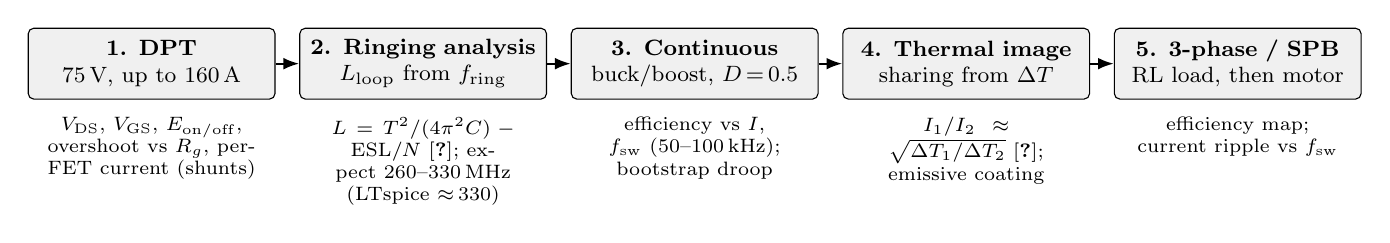
\begin{tikzpicture}[node distance=3mm,font=\small]
\node[hw,text width=2.9cm,font=\footnotesize] (a) {\textbf{1. DPT}\\75\,V, up to 160\,A};
\node[hw,text width=2.9cm,font=\footnotesize,right=of a] (b) {\textbf{2. Ringing analysis}\\$L_\mathrm{loop}$ from $f_\mathrm{ring}$};
\node[hw,text width=2.9cm,font=\footnotesize,right=of b] (c) {\textbf{3. Continuous}\\buck/boost, $D$\,=\,0.5};
\node[hw,text width=2.9cm,font=\footnotesize,right=of c] (d) {\textbf{4. Thermal image}\\sharing from $\Delta T$};
\node[hw,text width=2.9cm,font=\footnotesize,right=of d] (e) {\textbf{5. 3-phase / SPB}\\RL load, then motor};
\foreach \x/\y in {a/b,b/c,c/d,d/e} \draw[arr] (\x)--(\y);
\node[font=\scriptsize,text width=2.9cm,align=center,below=1mm of a] {$V_\mathrm{DS}$, $V_\mathrm{GS}$, $E_\mathrm{on/off}$, overshoot vs $R_g$, per-FET current (shunts)};
\node[font=\scriptsize,text width=2.9cm,align=center,below=1mm of b] {$L=T^2/(4\pi^2C)-\mathrm{ESL}/N$~\cite{tran2025}; expect 260--330\,MHz (LTspice $\approx$\,330)};
\node[font=\scriptsize,text width=2.9cm,align=center,below=1mm of c] {efficiency vs $I$, $f_\mathrm{sw}$ (50--100\,kHz); bootstrap droop};
\node[font=\scriptsize,text width=2.9cm,align=center,below=1mm of d] {$I_1/I_2\approx\sqrt{\Delta T_1/\Delta T_2}$~\cite{cooke2026}; emissive coating};
\node[font=\scriptsize,text width=2.9cm,align=center,below=1mm of e] {efficiency map; current ripple vs $f_\mathrm{sw}$};
\end{tikzpicture}
\caption{Validation sequence and what each step verifies.}\label{fig:valid}
\end{figure}
\textbf{Measurement requirements.} The turn-off edge takes about \Trise\,ns (\DvdtOff\,V/ns), and the cell loop rings at 260--330\,MHz (0.374\,nH with the $C_\mathrm{oss}$ of the off-state FET, 1.0\,nF at 50\,V to $\approx$\,0.6\,nF at 75\,V; LTspice shows $\approx$\,330\,MHz).
Probes and scope therefore need $\geq$\,1\,GHz bandwidth with MMCX or tip-and-barrel connections at the device pads~\cite{wattenberg2023}.
High-side $V_\mathrm{GS}$ needs an optically isolated probe.
As noted in~\cite{brothers2019}, terminal measurements under-read the die $V_\mathrm{DS}$, so the test points sit at the QL drain and source pads.

%=====================================================================
\section{Conclusions and next iteration}
%=====================================================================
The building block meets the efficiency target at 50\,kHz with a small margin once the switching-harmonic copper loss is included (\Eta\,\%), needs copper and capacitor-placement improvements for 100\,kHz (\EtaHundred\,\% today), and achieves a power-loop inductance below the reviewed designs, with equal loops and gate stars for the paralleled FETs.
The model-based flow makes the design reproducible and lets each change be traced to its effect on losses, overshoot and sharing.
Planned improvements, ranked by benefit:
\begin{enumerate}\itemsep1pt
\item Gate-bump mitigation (external $C_\mathrm{GS}$ or small negative bias; driver with Miller clamp), verified in the DPT.
\item Copper-loss reduction: DC busbar contacts next to each cell and heavier L3/L4 copper (about $-2$\,W), and more capacitance next to each cell to shorten the ripple path. This restores margin at 50\,kHz and brings 100\,kHz back to about 99.52\,\%.
\item A larger or film DC link if the shared-bus ripple must be held at $\pm$2\,\% across all operating points, and a separate 0.5--0.6\,mF bank for the DPT.
\item When the machine is selected, evaluate machine-side PWM losses in a separate study and confirm the switching frequency against the winding-ripple requirement.
\end{enumerate}

\begin{thebibliography}{99}\small
\bibitem{tran2025} M.~T.~Tran \emph{et al.}, ``A high-performance GaN power module with parallel packaging for high-current and low-voltage traction inverter applications,'' \emph{IEEE J. Emerg. Sel. Topics Power Electron.}, vol.~13, no.~1, pp.~1188--1209, Feb.~2025.
\bibitem{zou2025} M.~Zou \emph{et al.}, ``Systematic efficiency-density co-optimization of 100\,kW GaN traction inverter: methodology and integration,'' \emph{IEEE Trans. Power Electron.}, vol.~40, no.~11, pp.~16281--16299, Nov.~2025.
\bibitem{cooke2026} M.~W.~J.~Cooke and D.~J.~Rogers, ``120\,V, 155\,A traction inverter using eight parallel GaN HEMTs,'' 2026.
\bibitem{wattenberg2023} M.~Wattenberg, O.~G.~Lorenz, and J.~Sanchez, ``A multi-kilowatt low-profile GaN inverter for light electric vehicles and high-power tools,'' in \emph{Proc. IEEE APEC}, 2023, pp.~1443--1450.
\bibitem{lu2017} J.~Lu and D.~Chen, ``Paralleling GaN E-HEMTs in 10\,kW--100\,kW systems,'' in \emph{Proc. IEEE APEC}, 2017, pp.~3049--3056.
\bibitem{brothers2019} J.~A.~Brothers and T.~Beechner, ``GaN module design recommendations based on the analysis of a commercial 3-phase GaN module,'' in \emph{Proc. IEEE ECCE}, 2019, pp.~4109--4116.
\bibitem{musumeci2022} S.~Musumeci, V.~Barba, and M.~Palma, ``GaN-based low-voltage inverter for electric scooter drive system,'' in \emph{Proc. AEIT}, 2022.
\bibitem{palma2024} M.~Palma, V.~Barba, and S.~Musumeci, ``Parallel connection of GaN FETs: an experimental investigation approach,'' in \emph{Proc. PCIM Europe}, 2024, pp.~1563--1568.
\bibitem{satpathy2022} S.~Satpathy, P.~P.~Das, S.~Bhattacharya, and V.~Veliadis, ``Design considerations of a GaN-based three-level traction inverter for electric vehicles,'' in \emph{Proc. IEEE WiPDA}, 2022, pp.~192--197.
\bibitem{novo2024} D.~Novo \emph{et al.}, ``Development and testing of GaN power modules for EV traction inverters,'' in \emph{Proc. CIPS}, 2024, pp.~692--698.
\bibitem{rahman2025} M.~D.~Rahman \emph{et al.}, ``Design and evaluation of a 650\,V, 300\,A GaN-based power module with integrated drivers and ultra-low inductance layout,'' in \emph{Proc. IEEE WiPDA}, 2025.
\end{thebibliography}
\end{document}
